% Projekt dyplomowy — szablon WIMiIP/AGH (klasa aghthesis). Kompilacja: `make` (pdflatex → bibtex → pdflatex ×2).
\documentclass[polish,12pt]{aghthesis}
\usepackage[utf8]{inputenc}
\input{glyphtounicode}\pdfgentounicode=1
\usepackage{url}
\usepackage{array}
\usepackage{subcaption}
\usepackage{hyperref}
\hypersetup{colorlinks, citecolor=black, filecolor=black, linkcolor=black, urlcolor=black}
\usepackage{enumitem}
\usepackage{tabularx}
\usepackage{float}
\usepackage{placeins}
\usepackage{algorithm}
\usepackage{algpseudocode}
\usepackage{listings}
\usepackage{doi}
\usepackage{booktabs}   % tabele z results/evaluation.tex
\usepackage{amsmath}
\usepackage{caption}    % \captionof
\usepackage{tikz}
\usetikzlibrary{shapes.geometric,shapes.multipart,arrows.meta,positioning,fit,calc}
% Wspólny styl diagramów TikZ (wczytywany raz w main.tex)
\definecolor{dgBox}{HTML}{F3F4F6}
\definecolor{dgLine}{HTML}{4B5563}
\definecolor{dgPkg}{HTML}{EEF2FF}
\definecolor{dgPkgLine}{HTML}{4F46E5}
\definecolor{dgLib}{HTML}{ECFDF5}
\definecolor{dgLibLine}{HTML}{0D9488}
\definecolor{dgExt}{HTML}{FFF7ED}
\definecolor{dgExtLine}{HTML}{D97706}
\definecolor{dgHead}{HTML}{E0E7FF}
\tikzset{
  dg/.style={font=\footnotesize, line width=.5pt, >={Stealth[length=2mm, width=1.6mm]}},
  box/.style={draw=dgLine, fill=dgBox, rounded corners=3pt, align=center, inner sep=5pt, minimum height=8mm},
  pkg/.style={box, draw=dgPkgLine, fill=dgPkg, minimum width=26mm, minimum height=11mm},
  lib/.style={box, draw=dgLibLine, fill=dgLib, minimum width=26mm, minimum height=11mm},
  ext/.style={box, draw=dgExtLine, fill=dgExt, minimum width=26mm, minimum height=11mm},
  actor/.style={box, minimum width=22mm},
  uc/.style={draw=dgLine, fill=white, ellipse, align=center, inner sep=2pt, minimum width=44mm, minimum height=9mm},
  flow/.style={->, draw=dgLine, line width=.7pt},
  ctl/.style={->, draw=dgPkgLine, line width=.7pt, dashed},
  dep/.style={-, draw=dgLine!50, line width=.5pt},
  lbl/.style={font=\scriptsize, fill=white, inner sep=1.5pt, text=dgLine},
}


% ---------- listingi ----------
\definecolor{codegreen}{rgb}{0,0.6,0}
\definecolor{codegray}{rgb}{0.5,0.5,0.5}
\definecolor{codepurple}{rgb}{0.58,0,0.82}
\definecolor{backcolour}{rgb}{0.95,0.95,0.92}

\lstdefinestyle{mystyle}{
   backgroundcolor=\color{backcolour},
   commentstyle=\color{codegreen},
   keywordstyle=\color{magenta},
   numberstyle=\tiny\color{codegray},
   stringstyle=\color{codepurple},
   basicstyle=\ttfamily\footnotesize,
   breakatwhitespace=false, breaklines=true, captionpos=b, keepspaces=true,
   numbers=left, numbersep=5pt, showspaces=false, showstringspaces=false,
   showtabs=false, tabsize=2,
   literate={ą}{{\k{a}}}1 {ć}{{\'c}}1 {ę}{{\k{e}}}1 {ł}{{\l{}}}1 {ń}{{\'n}}1
            {ó}{{\'o}}1 {ś}{{\'s}}1 {ź}{{\'z}}1 {ż}{{\.z}}1
            {Ą}{{\k{A}}}1 {Ć}{{\'C}}1 {Ę}{{\k{E}}}1 {Ł}{{\L{}}}1 {Ń}{{\'N}}1
            {Ó}{{\'O}}1 {Ś}{{\'S}}1 {Ź}{{\'Z}}1 {Ż}{{\.Z}}1
}

\lstdefinelanguage{TypeScript}{
    keywords={break, case, catch, class, const, continue, debugger, default, delete, do, else,
      export, finally, for, function, if, import, in, instanceof, new, return, super, switch,
      this, throw, try, typeof, var, void, while, with, yield, async, await, let, from, as,
      interface, type, enum, implements, extends, readonly, public, private, protected, static,
      declare, namespace, keyof, satisfies},
    keywordstyle=\color{magenta}\bfseries,
    ndkeywords={Promise, console, JSON, Error, Boolean, Number, String, Object, Function, Array,
      Date, RegExp, Map, Set, Infinity, NaN, undefined, null, bigint, number, string, boolean,
      unknown, never, any, BigInt},
    ndkeywordstyle=\color{teal}\bfseries,
    identifierstyle=\color{black},
    sensitive=true,
    comment=[l]{//}, morecomment=[s]{/*}{*/},
    commentstyle=\color{codegreen}\ttfamily,
    stringstyle=\color{codepurple}\ttfamily,
    morestring=[b]', morestring=[b]", morestring=[b]`,
}

\lstset{style=mystyle}
\renewcommand{\lstlistingname}{Fragment kodu}
\captionsetup[lstlisting]{justification=raggedright, singlelinecheck=false}

% ---------- metadane ----------
\author{Kacper Kończyk}                         % TODO: zweryfikować pisownię jak w USOS
\department{KATEDRA INFORMATYKI STOSOWANEJ I MODELOWANIA} % TODO: potwierdzić katedrę opiekuna
\titlePL{Projekt systemu komputerowego do analizy danych transakcyjnych w~celu wykrywania
  rozbieżności cenowych oraz heurystycznej oceny wykonalności arbitrażu w~zdecentralizowanych
  giełdach}
\titleEN{Design of a~computer system for the analysis of transactional data to detect price
  discrepancies and to heuristically assess the feasibility of arbitrage on decentralized
  exchanges}
\fieldofstudy{Informatyka Techniczna}
\supervisor{dr hab. inż. Zbigniew Mitura}
\date{2026}

\raggedbottom
\renewcommand{\topfraction}{.9}\renewcommand{\textfraction}{.05}\renewcommand{\floatpagefraction}{.85}
\begin{document}
\maketitle
\tableofcontents

\newpage
\section{Wstęp}
\subsection{Kontekst i~motywacja}

Zdecentralizowane giełdy (ang. \emph{decentralized exchange}, DEX) umożliwiają wymianę aktywów
cyfrowych za pomocą smart kontraktów. Znacząca część z~tych giełd korzysta z~algorytmu AMM
(ang. \emph{automated market maker}). Ponieważ różne rynki mają niezależne pule płynności,
istnieje możliwość występowania rozbieżności cenowych pomiędzy tymi samymi aktywami.

W~takim przypadku pojawia się możliwość arbitrażu: zakupu aktywu na tańszym rynku i~sprzedaży na
droższym. Dzięki wykorzystaniu tego zjawiska rynki stają się bardziej efektywne: znikają
rozbieżności cenowe. Sama różnica cenowa nie oznacza jednak, że taka okazja jest wykonalna.
Wpływają na nią takie czynniki jak koszty wykonania transakcji, płynność czy kolejność wykonania
transakcji, która w~warunkach konkurencji może ulegać zmianie poprzez mechanizmy znane jako MEV
(ang. \emph{miner extractable value}). W~konsekwencji samo wykrycie rozbieżności cenowej nie
jest wystarczające do oceny możliwości jej wykorzystania w~praktyce. Konieczna jest analiza
czynników wpływających na wykonalność takich okazji, co może stanowić podstawę opracowania
narzędzi analitycznych zabezpieczających potencjalnych uczestników rynku (np. animatorów
rynku), tak aby ich oferty nie były narażone na straty.

\subsection{Cel i~zakres pracy}

Celem projektu jest opracowanie i~implementacja systemu zbierającego i~analizującego
historyczne dane ze zdecentralizowanych giełd w~celu wykrywania rozbieżności cenowych oraz
oceny wykonalności takich okazji. Ma on pełnić rolę narzędzia analitycznego zabezpieczającego
uczestników rynku przy realizacji strategii cenowych. W~ramach projektu opracowano
heurystyczny algorytm oceny wykonalności wykrytych okazji arbitrażowych.

Heurystyczna ocena wykonalności stanowi punkt wyjścia: w~pracy zestawiono prostą heurystykę
progową z~jej wersją skalibrowaną na danych historycznych oraz z~dwoma modelami opartymi na
logice rozmytej, systemem wnioskowania Mamdaniego, którego reguły zapisują wiedzę ekspercką
o~czynnikach wykonalności, oraz siecią neuro-rozmytą ANFIS, w~której parametry reguł są uczone
z~danych. Porównanie tych modeli na wspólnym protokole ewaluacji, z~etykietami uzyskanymi przez
retrospektywną weryfikację on-chain, pozwala ocenić, w~jakim stopniu ocena wykonalności może
być trafniejsza od samego wykrycia rozbieżności cenowej.

Realizacja celu obejmuje następujące zadania:
\begin{itemize}[nosep]
  \item zaprojektowanie i~implementację systemu gromadzącego historyczne stany puli Uniswap~V2
        i~Sushiswap z~węzła Ethereum oraz wykrywającego rozbieżności cenowe,
  \item zbudowanie procedury weryfikacji retrospektywnej, ustalającej, czy rozbieżność została
        skonsumowana on-chain,
  \item opracowanie heurystycznego algorytmu oceny wykonalności i~porównanie go z~modelami
        rozmytymi (system Mamdaniego, ANFIS) na wspólnym protokole ewaluacji,
  \item udostępnienie wyników w~interaktywnym panelu, w~tym w~trybie analizy bieżących danych.
\end{itemize}

\subsection{Założenia techniczne}

Przedmiotem analizy jest sieć Ethereum (mainnet) oraz dwie giełdy działające w~modelu AMM
o~stałym iloczynie: Uniswap~V2 i~Sushiswap. Obie mają identyczne kontrakty puli, tę samą
prowizję i~te same zdarzenia, więc rozbieżność cenową między nimi można liczyć wprost
z~rezerw w~tym samym bloku. Badanie objęło cztery pary tokenów (WETH/USDC, WETH/USDT,
WETH/DAI, WBTC/WETH) w~czterech dwutygodniowych oknach historycznych z~lat 2021--2022,
dobranych tak, aby obejmowały okresy gwałtownych ruchów cen (krach z~maja 2021~r., szczyt
z~listopada 2021~r., upadek Terra/Luna w~maju 2022~r., upadek FTX w~listopadzie 2022~r.).
Okno majowe 2021~r. poprzedza zmianę EIP-1559, pozostałe są po niej, co pozwala sprawdzić
modele w~dwóch reżimach opłat.

Dane pochodzą wyłącznie z~archiwalnego węzła Ethereum przez interfejs JSON-RPC: logi zdarzeń
kontraktów puli (\texttt{eth\_getLogs}), metadane bloków i~paragony transakcji. We wniosku
o~zatwierdzenie tematu przewidziano indeksowanie danych subgraphami usługi The Graph
i~udostępnianie ich backendowi w~postaci zapytań GraphQL. W~trakcie projektowania odstąpiono od
tego rozwiązania z~trzech powodów. Po pierwsze, publiczne subgraphy Uniswap~V2 i~Sushiswap
agregują stan puli w~przedziałach godzinowych i~dziennych, a~ocena wykonalności wymaga rezerw
po każdym bloku. Po drugie, weryfikacja retrospektywna okazji potrzebuje paragonów transakcji
konsumujących (logi \texttt{Transfer}, zużyty gaz), których subgraph nie udostępnia, więc
dostęp do węzła RPC był niezbędny niezależnie od źródła stanów. Po trzecie, logi zdarzeń są
źródłem pierwotnym, z~którego subgraph sam jest budowany; pobranie ich bezpośrednio usuwa
zależność od usługi zewnętrznej i~upraszcza reprodukcję wyników. Pozostałe założenia
z~wniosku zachowano: analizowane są zdarzenia smart kontraktów giełd AMM w~sieci zgodnej
z~EVM, system napisano w~języku TypeScript, a~dane przechowuje relacyjna baza PostgreSQL.

Przyjęto, że transakcja arbitrażowa to atomowa wymiana w~dwóch pulach tej samej pary w~jednej
transakcji (dwa swapy i~transfer, ok. 220\,000 jednostek gazu), a~okazją jest blok, w~którym
rozbieżność przekracza sumę prowizji obu wymian. Arbitraż trójkątny, wielohopowy i~między
sieciami pozostaje poza zakresem. System jest aplikacją lokalną, bez uwierzytelniania
i~bez obsługi reorganizacji łańcucha; analizowane bloki są dawno finalne.

\subsection{Zakres prac własnych a~elementy wykorzystane}

W~ramach projektu zaprojektowano i~zaimplementowano od podstaw: schemat bazy danych
i~migracje; warstwę pobierania danych z~węzła RPC (porcjowanie, wznawianie, rotacja węzłów);
odtwarzanie stanu puli po każdym bloku i~arytmetykę AMM na liczbach całkowitych, w~tym wzór
na optymalną wielkość transakcji; obliczanie cech i~wykrywanie okazji; procedurę weryfikacji
retrospektywnej z~klasyfikacją statusu, beneficjenta i~trasy; heurystykę progową oraz jej
wersję kalibrowaną; implementację ANFIS z~uczeniem gradientowym; protokół ewaluacji
z~podziałem grupowym, bootstrapem i~metrykami; kolejkę zadań, serwer API i~interfejs
użytkownika z~trybem na żywo; zestaw 953 testów automatycznych, potok CI i~skrypty
reprodukcji.

Zdefiniowano cechy $S$, $G$, $L$, $M$
oraz bazę 16 reguł i~parametry termów systemu Mamdaniego, który w~tej pracy zaimplementowano jako moduł oceny i~poddano ewaluacji na etykietach z~weryfikacji. Do wnioskowania
rozmytego użyto biblioteki \texttt{@thi.ng/fuzzy}, do warstwy danych Drizzle ORM i~PostgreSQL,
do API Fastify, do walidacji kontraktów zod, do interfejsu React, Vite, TanStack Query
i~Recharts, a~do testów Vitest. Dekodowanie logów kontraktów oparto na bibliotece ethers.
Wzory arytmetyki puli odtworzono z~kontraktów Uniswap~V2. Narzędzia generatywnej sztucznej inteligencji użyte przy
realizacji projektu opisano w~rozdziale~6.

\subsection{Struktura pracy i~konwencja edytorska}

Rozdział~2 wprowadza pojęcia z~zakresu Ethereum, giełd AMM, arbitrażu i~MEV, logiki rozmytej
oraz oceny klasyfikatorów, a~kończy się przeglądem istniejących rozwiązań i~uzasadnieniem
własnego podejścia. Rozdział~3 opisuje projekt i~implementację systemu: przypadki użycia,
architekturę, model danych, pozyskiwanie danych, wykrywanie okazji, cztery modele oceny,
weryfikację retrospektywną, kolejkę zadań, API i~interfejs. Rozdział~4 przedstawia zbiór
danych, protokół ewaluacji, sprawdzenie poprawności implementacji, porównanie modeli, ich
stabilność oraz wstępną ocenę ekonomiczną, a~zamyka go dyskusja wyników i~ograniczeń.
Rozdział~5 podsumowuje realizację celów i~wskazuje kierunki dalszych prac, rozdział~6
dokumentuje użycie narzędzi GenAI. Załączniki zawierają instrukcję uruchomienia, słownik
pojęć, pełną bazę reguł, opis repozytorium i~listę punktów końcowych API.

W~tekście nazwy plików, tabel, kolumn, zmiennych i~poleceń zapisano czcionką o~stałej
szerokości (np. \texttt{block\_states}, \texttt{eth\_getLogs}), terminy angielskie kursywą
z~podaniem polskiego odpowiednika przy pierwszym wystąpieniu, a~fragmenty kodu źródłowego
TypeScript i~polecenia powłoki jako numerowane listingi (,,Fragment kodu''). Wzory są
numerowane w~nawiasach okrągłych, a~odwołania do literatury podano w~nawiasach kwadratowych
w~kolejności cytowania. Liczby w~tekście zapisano z~przecinkiem dziesiętnym i~odstępem jako
separatorem tysięcy; kwoty w~USD podano według kursu ETH/USD z~bloku, którego dotyczą.

\newpage
\section{Giełdy zdecentralizowane i~arbitraż --- przegląd zagadnień}

\subsection{Ethereum: bloki, transakcje, zdarzenia i~opłaty za gaz}

Ethereum jest zdecentralizowaną maszyną stanów. Stan globalny zmieniają wyłącznie transakcje
zgrupowane w~bloki, a~semantykę ich wykonania definiuje maszyna wirtualna EVM
(ang. \emph{Ethereum Virtual Machine})~\cite{ethereum_yellowpaper}. Kontrakt może podczas wykonania
wyemitować \emph{zdarzenie} (ang. \emph{event}), które trafia do paragonu transakcji jako
\emph{log}: adres kontraktu, do czterech indeksowanych tematów (ang. \emph{topics}) i~dane.
Węzły udostępniają metodę JSON-RPC \texttt{eth\_getLogs}, pobierającą logi z~zakresu bloków według
adresu i~tematu. Kontrakty giełd emitują zdarzenie po każdej zmianie rezerw, więc logi są
kompletnym i~weryfikowalnym zapisem historii puli. Na tej własności opiera się warstwa
pozyskiwania danych z~rozdziału~3.4.

Każda operacja EVM ma koszt wyrażony w~jednostkach \emph{gazu}. Nadawca deklaruje limit gazu
i~cenę za jednostkę. W~pierwotnym modelu opłat cena gazu była pojedynczą wartością
\texttt{gasPrice} ustalaną przez nadawcę; górnicy porządkowali transakcje malejąco według tej
ceny, co sprowadzało dostęp do bloku do jawnej licytacji. Zmiana EIP-1559~\cite{eip1559},
aktywowana w~bloku 12\,965\,000 (5~sierpnia 2021~r.), wprowadziła opłatę bazową
\texttt{baseFeePerGas}, ustalaną przez protokół i~spalaną, oraz napiwek
\texttt{maxPriorityFeePerGas} dla producenta bloku. Z~analizy Liu i~in.~\cite{liu_eip1559} wynika,
że EIP-1559 zmniejszyło rozrzut cen gazu wewnątrz bloku i~ułatwiło ich szacowanie, ale samego
poziomu opłat istotnie nie obniżyło. Dla tej pracy oznacza to dwie rzeczy: koszt transakcji
arbitrażowej trzeba szacować inaczej w~oknach sprzed i~po EIP-1559 (rozdział~3.4), a~cena gazu
pozostaje wielkością zmienną w~czasie i~jednym z~głównych składników kosztu arbitrażu.

\subsection{Automatyczni animatorzy rynku o~stałym iloczynie}

Giełda typu AMM zastępuje księgę zleceń pulą płynności. Kontrakt przechowuje rezerwy dwóch
tokenów i~wycenia wymianę deterministyczną funkcją tych rezerw; kontrahentem każdej transakcji
jest sama pula~\cite{xu_sok_amm}. W~protokole Uniswap~V2~\cite{uniswap_v2} funkcją tą jest stały
iloczyn. Dla rezerw $x$ i~$y$ tokenów $X$ i~$Y$ niezmiennik ma postać
\begin{equation}
  x \cdot y = k .
  \label{eq:cpmm}
\end{equation}
Cena chwilowa tokena $X$ wyrażona w~tokenie $Y$ wynika ze stosunku rezerw:
\begin{equation}
  p = \frac{y}{x}.
  \label{eq:spot}
\end{equation}
Wymiana $\Delta x$ jednostek $X$ przy prowizji $\varphi = 0{,}3\,\%$ zwraca
\begin{equation}
  \Delta y = \frac{(1-\varphi)\,\Delta x \cdot y}{x + (1-\varphi)\,\Delta x}
           = \frac{997\,\Delta x\, y}{1000\,x + 997\,\Delta x},
  \label{eq:amountout}
\end{equation}
zgodnie z~funkcją \texttt{getAmountOut} w~kontraktach Uniswap~V2. Z~równań \eqref{eq:cpmm} i~\eqref{eq:amountout} widać, że cena efektywna rośnie z~wielkością transakcji (poślizg cenowy),
a~prowizja zostaje w~puli i~powiększa $k$. Po każdej zmianie stanu kontrakt pary emituje
zdarzenie \texttt{Sync} z~nowymi rezerwami, a~przy wymianie dodatkowo \texttt{Swap} z~kwotami.
Cenę~\eqref{eq:spot} w~dowolnym bloku można więc odtworzyć z~samych logów.

Sushiswap powstał w~2020~r. jako kopia (ang. \emph{fork}) kontraktów Uniswap~V2 z~własnymi pulami
płynności. Oba protokoły mają identyczną formułę~\eqref{eq:amountout}, te same sygnatury zdarzeń
i~tę samą prowizję, więc porównanie ich cen sprowadza się do porównania rezerw w~tym samym
bloku. Systematyczny przegląd protokołów AMM, także tych o~stałej średniej i~o~skoncentrowanej
płynności, zawiera praca Xu i~in.~\cite{xu_sok_amm}.

Angeris i~in.~\cite{angeris_uniswap} pokazali, że w~rynku o~stałym iloczynie każde odchylenie
ceny~\eqref{eq:spot} od ceny referencyjnej tworzy zyskowną okazję dla arbitrażysty, a~zysk ten
maksymalizuje transakcja zamykająca odchylenie do poziomu prowizji. Przy dostatecznej
aktywności arbitrażystów cena puli musi zatem śledzić rynek referencyjny. Obserwowana
rozbieżność między dwiema pulami świadczy o~czymś przeciwnym: w~danym bloku arbitraż nie został
jeszcze wykonany.

\subsection{Arbitraż między pulami i~czynniki jego wykonalności}

Niech dwie pule tej samej pary tokenów, $A$ i~$B$, mają ceny chwilowe $p_A$ i~$p_B$. Względną
rozbieżność cenową definiuje się jako
\begin{equation}
  S = \frac{|p_A - p_B|}{\min(p_A, p_B)} \cdot 100\,\%.
  \label{eq:spread}
\end{equation}
Arbitraż dwupulowy to zakup tokena w~puli tańszej i~sprzedaż w~droższej w~jednej, atomowej
transakcji. Każda z~dwóch wymian jest obciążona prowizją $\varphi$, więc zysk brutto pojawia się
dopiero, gdy rozbieżność przekracza koszt prowizji obu nóg, $(1-\varphi)^{-2} - 1 \approx
0{,}60\,\%$. W~pracy przyjęto próg $0{,}65\,\%$ (rozdział~3.5). Dla ustalonego stanu obu puli
istnieje wielkość transakcji maksymalizująca zysk brutto; wynika ona z~równania
\eqref{eq:amountout} i~jest wyprowadzona w~rozdziale~3.5.

Rozbieżność powyżej progu nie przesądza jednak o~wykonalności. Literatura wskazuje trzy grupy
czynników. Pierwszą jest koszt wykonania: transakcja arbitrażowa zużywa gaz na dwie wymiany
i~transfery, a~przy wysokiej cenie gazu ten koszt stały może przewyższyć zysk brutto. Drugą jest
płynność. Zysk z~rozbieżności ogranicza poślizg, więc w~płytkich pulach optymalna transakcja
jest mała, a~zysk absolutny niewielki~\cite{angeris_uniswap}. Trzecią grupą jest konkurencja
i~kolejność transakcji: okazję widzą wszyscy obserwatorzy sieci, a~o~tym, kto ją zrealizuje,
decyduje kolejność w~bloku.

Ostatni czynnik jest przedmiotem badań nad wartością możliwą do wydobycia przez producenta
bloku (ang. \emph{miner/maximal extractable value}, MEV). Daian i~in.~\cite{daian_flashboys}
udokumentowali boty arbitrażowe konkurujące o~pierwszeństwo w~bloku przez licytację ceny gazu
(ang. \emph{priority gas auctions}); znaczna część zysku z~arbitrażu trafia wtedy do górników,
a~sama konkurencja destabilizuje konsensus. Zhou i~in.~\cite{zhou_hft_dex} sformalizowali ataki na
kolejność transakcji na giełdach AMM (\emph{front-running}, \emph{sandwich}), a~Qin
i~in.~\cite{qin_bev} oszacowali łączną skalę wartości wydobywanej z~DeFi, w~tym z~arbitrażu.
Wniosek istotny dla tej pracy: aktywność botów i~podwyższona cena gazu w~danym momencie
zmniejszają szansę, że obserwator rozbieżności skonsumuje ją jako pierwszy. Te dwie wielkości
tworzą cechę ryzyka~$M$ w~rozdziale~3.5. Odkąd Flashbots udostępnili prywatny kanał przekazywania
transakcji do górników~\cite{flashbots}, część konkurencji przeniosła się poza publiczną pulę
transakcji, co dodatkowo utrudnia ocenę wykonalności na podstawie samych danych on-chain.
Propozycje ograniczania takich manipulacji na poziomie protokołu omawiają m.in. Heimbach
i~Wattenhofer~\cite{heimbach_sandwich}.

Badania empiryczne potwierdzają, że rozbieżności między pulami występują i~są konsumowane na dużą
skalę. McLaughlin i~in.~\cite{mclaughlin_arbitrage} w~pomiarze obejmującym 28~miesięcy
zidentyfikowali 3{,}8~mln wykonanych arbitraży o~łącznym zysku ok.~321~mln USD. Zaobserwowali też,
że część okazji utrzymuje się przez kilka kolejnych bloków. Berg i~in.~\cite{berg_inefficiencies}
analizowali pary Uniswap i~Sushiswap i~wykazali, że efektywność cenowa obu giełd spada w~okresach
wysokiej zmienności kursów, a~liczba okazji arbitrażu cyklicznego wówczas rośnie. Metodę
identyfikacji arbitraży cyklicznych w~Uniswap~V2 z~danych on-chain opisali Wang
i~in.~\cite{wang_cyclic_arbitrage}. Z~tych obserwacji wynikają dwie decyzje projektowe: dobór okien
historycznych obejmujących gwałtowne ruchy cen oraz śledzenie konsumpcji okazji przez kilka
bloków po jej wykryciu (rozdział~3.7).

\subsection{Logika rozmyta i~systemy wnioskowania rozmytego}

Zbiór rozmyty $\tilde{A}$ w~przestrzeni $U$ jest określony funkcją przynależności
$\mu_{\tilde A}\colon U \to [0,1]$~\cite{zadeh1965}. W~odróżnieniu od zbioru klasycznego element
może należeć do niego częściowo. Pojęcia nieostre, takie jak ,,duża rozbieżność'' czy ,,zaporowy
koszt gazu'', da się wtedy opisać funkcjami ciągłymi zamiast sztywnych progów. Dla oceny
wykonalności jest to naturalne: poszczególne czynniki nie mają ostrych granic i~wzajemnie się
kompensują.

System wnioskowania rozmytego typu Mamdaniego~\cite{mamdani1975} składa się z~bazy reguł postaci
,,\textsc{jeżeli} $x_1$ jest $\tilde A_1$ \textsc{i} $x_2$ jest $\tilde A_2$ \textsc{to} $y$ jest
$\tilde B$'', bloku rozmywania wejść, mechanizmu wnioskowania i~bloku wyostrzania. Stopień
aktywacji reguły oblicza t-norma (w~pracy minimum) stopni przynależności przesłanek. Konkluzja
reguły jest obcinana na tym poziomie (implikacja minimum), konkluzje wszystkich reguł agreguje
s-norma (maksimum), a~wynik liczbowy wyznacza środek ciężkości zagregowanego zbioru:
\begin{equation}
  y^{*} = \frac{\int y\, \mu_{\mathrm{agg}}(y)\, \mathrm{d}y}{\int \mu_{\mathrm{agg}}(y)\, \mathrm{d}y}.
  \label{eq:centroid}
\end{equation}
Zaletą modelu Mamdaniego jest interpretowalność. Reguły zapisują wiedzę ekspercką wprost, można
je czytać i~poprawiać bez danych uczących. Wadą jest brak mechanizmu strojenia: parametry funkcji
przynależności i~zestaw reguł dobiera się ręcznie. System Mamdaniego jako doradcę transakcyjnego
na rynku kryptowalut, z~regułami strojonymi algorytmem genetycznym, przedstawili Tupinambás
i~in.~\cite{tupinambas_fuzzy_crypto}.

Model Takagiego--Sugeno~\cite{takagi_sugeno1985} zachowuje rozmyte przesłanki, ale konkluzją reguły
$i$ jest funkcja wejść, w~wariancie pierwszego rzędu liniowa:
\begin{equation}
  y_i = c_{i0} + \sum_{j} c_{ij}\, x_j ,
  \qquad
  y = \frac{\sum_i w_i\, y_i}{\sum_i w_i},
  \label{eq:ts}
\end{equation}
gdzie $w_i$ jest stopniem aktywacji reguły. Wyjście~\eqref{eq:ts} jest ważoną średnią konkluzji,
przez co model jest różniczkowalny względem parametrów. Jang~\cite{jang1993} zaproponował ANFIS
(ang. \emph{adaptive-network-based fuzzy inference system}): model Takagiego--Sugeno zapisany jako
pięciowarstwowa sieć adaptacyjna (rozmywanie, iloczyn przesłanek, normalizacja aktywacji,
konkluzje liniowe, sumowanie) i~uczony algorytmem hybrydowym. Parametry konkluzji $c_{ij}$
wyznacza metoda najmniejszych kwadratów przy ustalonych przesłankach, a~parametry funkcji
przynależności koryguje krok gradientowy. ANFIS łączy czytelną strukturę regułową ze zdolnością
dopasowania do danych, kosztem częściowej utraty interpretowalności konkluzji. W~pracy oba
podejścia porównano na tym samym zestawie cech: system Mamdaniego z~regułami zapisanymi na
podstawie wiedzy dziedzinowej oraz ANFIS uczony na etykietach z~weryfikacji retrospektywnej
(rozdział~3.6).

\subsection{Ocena klasyfikatorów przy silnej nierównowadze klas}

Modele oceny wykonalności zwracają wynik liczbowy, który po przyłożeniu progu staje się decyzją
binarną. Ocena takich modeli wymaga miar niezależnych od progu i~odpornych na nierównowagę klas.
W~analizowanych danych okazje faktycznie skonsumowane stanowią około jednej dziesiątej
wykrytych rozbieżności.

Krzywa ROC (ang. \emph{receiver operating characteristic}) przedstawia zależność czułości od odsetka
fałszywych alarmów dla wszystkich progów. Pole pod nią (AUC) ma interpretację prawdopodobieństwa,
że losowo wybrany przykład pozytywny otrzyma wyższy wynik niż losowo wybrany
negatywny~\cite{fawcett2006}. Przy skośnym rozkładzie klas ROC bywa zbyt optymistyczna, bo duża
liczba negatywów maskuje fałszywe alarmy. Davis i~Goadrich~\cite{davis_goadrich2006} oraz Saito
i~Rehmsmeier~\cite{saito_pr_auc} pokazują, że krzywa precyzja--czułość i~pole pod nią (PR-AUC,
równoważne średniej precyzji) lepiej oddają użyteczność modelu, gdy liczy się jakość wskazań
pozytywnych. W~rozdziale~4 raportowane są obie miary, uzupełnione o~precyzję, czułość i~miarę
$F_1$ przy stałym progu. Niepewność AUC wyznaczono metodą bootstrap~\cite{efron1979}:
wielokrotne losowanie ze zwracaniem zbioru testowego daje rozkład statystyki, z~którego
odczytuje się przedział ufności. Sąsiednie bloki tej samej okazji są silnie skorelowane, a~jedna
transakcja może konsumować kilka rozbieżności, dlatego podział na zbiory uczący i~testowy musi
przebiegać na poziomie grup, nie pojedynczych obserwacji. Protokół opisano w~rozdziale~4.2.

\subsection{Istniejące rozwiązania i~uzasadnienie własnego podejścia}

Prace najbliższe tematycznie dzielą się na trzy grupy. Pierwszą stanowią pomiary ex post
wykonanych arbitraży i~MEV na podstawie historii łańcucha. McLaughlin
i~in.~\cite{mclaughlin_arbitrage} zbudowali system identyfikujący zrealizowane arbitraże oraz
detektor okazji obsługujący złożone modele cen; Qin i~in.~\cite{qin_bev} skwantyfikowali wartość
wydobytą z~różnych klas transakcji; narzędzie \emph{mev-inspect} Flashbots~\cite{mev_inspect}
klasyfikuje transakcje MEV w~zadanym zakresie bloków. Drugą grupę tworzą badania efektywności
rynku: Berg i~in.~\cite{berg_inefficiencies} mierzą, jak dokładnie Uniswap i~Sushiswap śledzą cenę
referencyjną, a~Wang i~in.~\cite{wang_cyclic_arbitrage} badają arbitraż cykliczny. Trzecią są
prace teoretyczne o~optymalnym arbitrażu w~rynkach o~stałej funkcji~\cite{angeris_uniswap}.

Wszystkie te prace odpowiadają na pytanie, co się wydarzyło albo jaki zysk był teoretycznie
możliwy. Żadna nie formułuje oceny wykonalności okazji \emph{ex ante}, w~chwili jej wykrycia, na
podstawie cech obserwowalnych w~danym bloku, ani nie weryfikuje takiej oceny względem
faktycznej konsumpcji. Tę lukę wypełnia system z~rozdziału~3. Łączy on wykrywanie rozbieżności
z~retrospektywną weryfikacją, czy zostały skonsumowane, a~uzyskane etykiety wykorzystuje do
porównania czterech modeli oceny (prostej heurystyki, jej wersji skalibrowanej, systemu Mamdaniego
i~ANFIS) na wspólnym protokole ewaluacji. Wnioskowanie rozmyte wybrano na rdzeń oceny z~powodu
charakteru problemu: czynniki wykonalności (rozbieżność, koszt gazu, płynność, ryzyko
konkurencji) są nieostre i~wzajemnie się kompensują, a~interpretowalność reguł pozwala wyjaśnić
każdą ocenę użytkownikowi narzędzia.

\newpage
\section{Projekt i~implementacja systemu}

\subsection{Idea systemu i~przypadki użycia}

System \texttt{dex-arb-analyzer} jest narzędziem analitycznym dla jednego aktora, badacza rynku.
Realizuje jeden zasadniczy przepływ. Dla wybranej pary tokenów i~okna czasowego pobiera z~węzła
Ethereum historię obu puli (Uniswap~V2 i~Sushiswap), odtwarza ich stan po każdym bloku, wykrywa
bloki z~rozbieżnością cenową powyżej progu i~ocenia każdą taką okazję czterema modelami.
Następnie sprawdza w~historii łańcucha, czy okazja została faktycznie skonsumowana. Uzyskane
etykiety służą do kalibracji i~uczenia modeli oraz do ich porównania. Przypadki użycia
(rys.~\ref{fig:uc}) obejmują:
\begin{itemize}[nosep]
  \item zlecenie pobrania danych dla puli i~okna (\emph{ingest}) oraz śledzenie postępu zadania,
  \item zlecenie analizy pary w~oknie (stany bloków, okazje, oceny modeli),
  \item zlecenie weryfikacji retrospektywnej okazji,
  \item przegląd szeregów czasowych (ceny, rozbieżność, gaz, oceny) i~listy okazji z~podglądem
        szczegółów pojedynczej okazji, w~tym aktywacji reguł rozmytych,
  \item kalibrację heurystyki (baseline~v2) i~trening ANFIS na wybranych oknach,
  \item porównanie modeli (macierze pomyłek, krzywe ROC, histogramy ocen),
  \item obserwację bieżącego stanu puli w~trybie ,,na żywo''.
\end{itemize}
\begin{figure}[H]\centering% Diagram przypadków użycia
\begin{tikzpicture}[dg]
\node[actor] (badacz) at (0,1.0) {Badacz};
\node[actor] (worker) at (0,-6.3) {Proces\\\texttt{worker}};
\node[actor] (rpc) at (13.2,-1.9) {Węzeł RPC};

\foreach \i/\t in {1/{Zleć pobranie danych (pula, okno)}, 2/{Zleć analizę pary w~oknie},
                   3/{Zleć weryfikację okazji}, 4/{Przeglądaj szeregi i~okazje},
                   5/{Kalibruj / trenuj model}, 6/{Porównaj modele}, 7/{Obserwuj stan na żywo}}
  \node[uc] (u\i) at (6.6, 2.9-1.15*\i) {\t};
\node[uc] (u8) at (6.6,-6.3) {Wykonaj zadanie z~kolejki};

\node[draw=dgLine, rounded corners=5pt, fit=(u1)(u8), inner sep=9pt] (box) {};
\node[anchor=south west, font=\footnotesize\ttfamily, text=dgLine] at ([yshift=1pt]box.north west) {dex-arb-analyzer};

\foreach \i in {1,...,7} \draw[dep, draw=dgLine] (badacz.east) -- (u\i.west);
\draw[dep, draw=dgLine] (worker.east) -- (u8.west);
\draw[ctl] (u8.north) -- node[lbl, right, xshift=2pt] {\textit{<<include>>} ingest, analiza, weryfikacja, trening} (u7.south);
\foreach \i in {1,3,7} \draw[dep, draw=dgLine] (rpc.west) -- (u\i.east);
\end{tikzpicture}

\caption{Diagram przypadków użycia systemu (opracowanie własne)}\label{fig:uc}\end{figure}

\subsection{Architektura}

System jest monorepozytorium npm (TypeScript, Node~$\geq$~20) złożonym z~ośmiu pakietów
o~rozłącznych odpowiedzialnościach (rys.~\ref{fig:arch}). Pakiet \texttt{core} zawiera arytmetykę
AMM, cechy, modele oceny i~metryki ewaluacji; jest to czysty kod bez dostępu do bazy i~sieci,
w~całości testowalny jednostkowo. Pakiet \texttt{db} definiuje schemat PostgreSQL (Drizzle ORM)
i~migracje, a~\texttt{shared} kontrakty danych (schematy zod) wspólne dla API i~interfejsu.
Za pobieranie zdarzeń i~bloków z~węzła RPC odpowiada \texttt{ingest}. Pakiet \texttt{analysis}
odtwarza stany, wykrywa okazje, ocenia je modelami, prowadzi weryfikację retrospektywną
i~buduje zbiór uczący. Zadania z~kolejki wykonuje \texttt{worker}, serwer HTTP (Fastify) to
\texttt{api}, a~interfejs użytkownika (React, Vite, TanStack Query, Recharts) to \texttt{web}.

Przepływ danych jest jednokierunkowy: RPC $\rightarrow$ \texttt{ingest} $\rightarrow$ baza
$\rightarrow$ \texttt{analysis} $\rightarrow$ baza $\rightarrow$ \texttt{api} $\rightarrow$
\texttt{web}. Zadania długotrwałe (pobieranie, analiza, weryfikacja, trening) nie są wykonywane
w~procesie API. Trafiają jako wiersze do tabeli \texttt{jobs} i~podejmuje je osobny proces
\texttt{worker}, więc interfejs pozostaje responsywny, a~zadania można wznowić po awarii. Każdy
krok jest idempotentny: ponowne uruchomienie nie duplikuje danych (wstawianie
z~\texttt{ON CONFLICT}, klucze naturalne).
\begin{figure}[H]\centering\resizebox{\linewidth}{!}{% Diagram komponentów i przepływu danych
\begin{tikzpicture}[dg, x=1cm, y=1cm,
  pkg/.append style={minimum width=28mm, minimum height=12mm},
  lib/.append style={minimum width=28mm, minimum height=12mm},
  ext/.append style={minimum width=28mm, minimum height=12mm}]
% rząd A: przepływ danych
\node[ext] (rpc)    at (0,0)  {Węzeł RPC\\(archiwalny)};
\node[pkg] (ingest) at (4,0)  {\texttt{ingest}};
\node[ext] (db)     at (8,0)  {PostgreSQL\\(dane, kolejka \texttt{jobs})};
\node[pkg] (api)    at (12,0) {\texttt{api}\\(Fastify)};
\node[pkg] (web)    at (16,0) {\texttt{web}\\(React)};
% rząd B
\node[pkg] (analysis) at (8,-3)  {\texttt{analysis}};
\node[lib] (core)     at (12,-3) {\texttt{core}\\(AMM, cechy, modele)};
\node[lib] (shared)   at (16,-3) {\texttt{shared}\\(DTO zod)};
% rząd C
\node[pkg] (worker) at (8,-6) {\texttt{worker}\\(wykonuje zadania)};

\draw[flow] (rpc) -- node[lbl,above] {logi, bloki} (ingest);
\draw[flow] (ingest) -- node[lbl,above] {zdarzenia} (db);
\draw[flow] (db) -- node[lbl,above] {SQL} (api);
\draw[flow] (api) -- node[lbl,above] {JSON} (web);
\draw[flow,<->] (db) -- node[lbl,right] {stany, okazje, oceny} (analysis);
\draw[flow] (rpc.south) |- node[lbl,pos=.75,above] {paragony transakcji} (analysis.west);
\draw[ctl] (worker) -- node[lbl,right] {uruchamia} (analysis);
\draw[ctl] (worker.west) -- ++(-4.6,0) |- node[lbl,pos=.22,right] {uruchamia} (ingest.west);
\draw[dep] (core) -- (analysis);
\draw[dep] (core) -- (api);
\draw[dep] (shared) -- (web);
\draw[dep] (shared) -- (core);

\node[font=\scriptsize, text=dgLine, anchor=west] at (-1.6,-7.4) {
  \tikz\draw[flow] (0,0)--(.5,0); przepływ danych\qquad
  \tikz\draw[ctl] (0,0)--(.5,0); sterowanie\qquad
  \tikz\draw[dep] (0,0)--(.5,0); zależność kodu};
\end{tikzpicture}
}
\caption{Architektura systemu: pakiety i~przepływ danych (opracowanie własne)}\label{fig:arch}\end{figure}

\subsection{Model danych}

Schemat bazy (rys.~\ref{fig:erd}) ma trzy warstwy. Warstwa konfiguracji to \texttt{dexes}
(giełdy z~adresem fabryki i~prowizją), \texttt{tokens}, \texttt{pairs} (para logiczna z~tokenem
bazowym i~kwotowanym), \texttt{pools} (pula danej giełdy dla pary; unikalna kombinacja
\texttt{(dex\_id, pair\_id)}) oraz \texttt{windows} (okno analizy z~zakresem czasu i~bloków).
Dane surowe przechowują tabele \texttt{blocks} (znacznik czasu, \texttt{base\_fee}, mediana ceny
gazu w~wei), \texttt{sync\_events} i~\texttt{swap\_events} z~kluczem naturalnym
\texttt{(pool\_id, block, log\_index)} oraz \texttt{ingest\_ranges}, czyli rejestr pobranych
zakresów bloków ze statusem, który zapewnia wznawialność. Dane pochodne to \texttt{block\_states}
(stan pary w~każdym bloku okna: ceny obu puli, rozbieżność, TVL, cechy $S,G,L,M$, optymalna
transakcja, zysk brutto; klucz \texttt{(pair\_id, block)}), \texttt{opportunities} (bloki
z~rozbieżnością powyżej progu), \texttt{opportunity\_verifications} (status, transakcja
konsumująca, zysk zrealizowany, koszt gazu, trasa, etykieta), \texttt{scoring\_models} (model
z~parametrami w~JSON, oknami treningowymi i~metrykami) i~\texttt{model\_scores} (ocena każdego
modelu dla każdego bloku). Kolejkę zadań reprezentuje tabela \texttt{jobs}.

Rezerwy i~kwoty tokenów są przechowywane jako \texttt{numeric(40,0)} i~przetwarzane
w~TypeScript jako \texttt{bigint}, żeby arytmetyka kontraktu była odtworzona dokładnie.
Wielkości w~USD i~cechy mają typ \texttt{double precision}. Poprawność danych wymuszają
ograniczenia \texttt{CHECK} (dwanaście w~migracji \texttt{0007}): zakresy cech ($S\in[0,3]$,
$G\in[0,2]$, $L\in[0,100]$, $M\in[0,100]$), zakres oceny modelu $[0,100]$,
$\texttt{blocks\_to\_consumption}\in[0,3]$ oraz równoważność ,,istnieje transakcja konsumująca''
$\Leftrightarrow$ ,,status jest konsumpcją''. Migracje są jednokierunkowe. Baza jest w~całości
odtwarzalna z~RPC, więc cofnięcie schematu oznacza odtworzenie bazy od zera.
\begin{figure}[H]\centering\resizebox{\linewidth}{!}{% Schemat bazy danych (uproszczony ERD). PK podkreślone, FK kursywą.
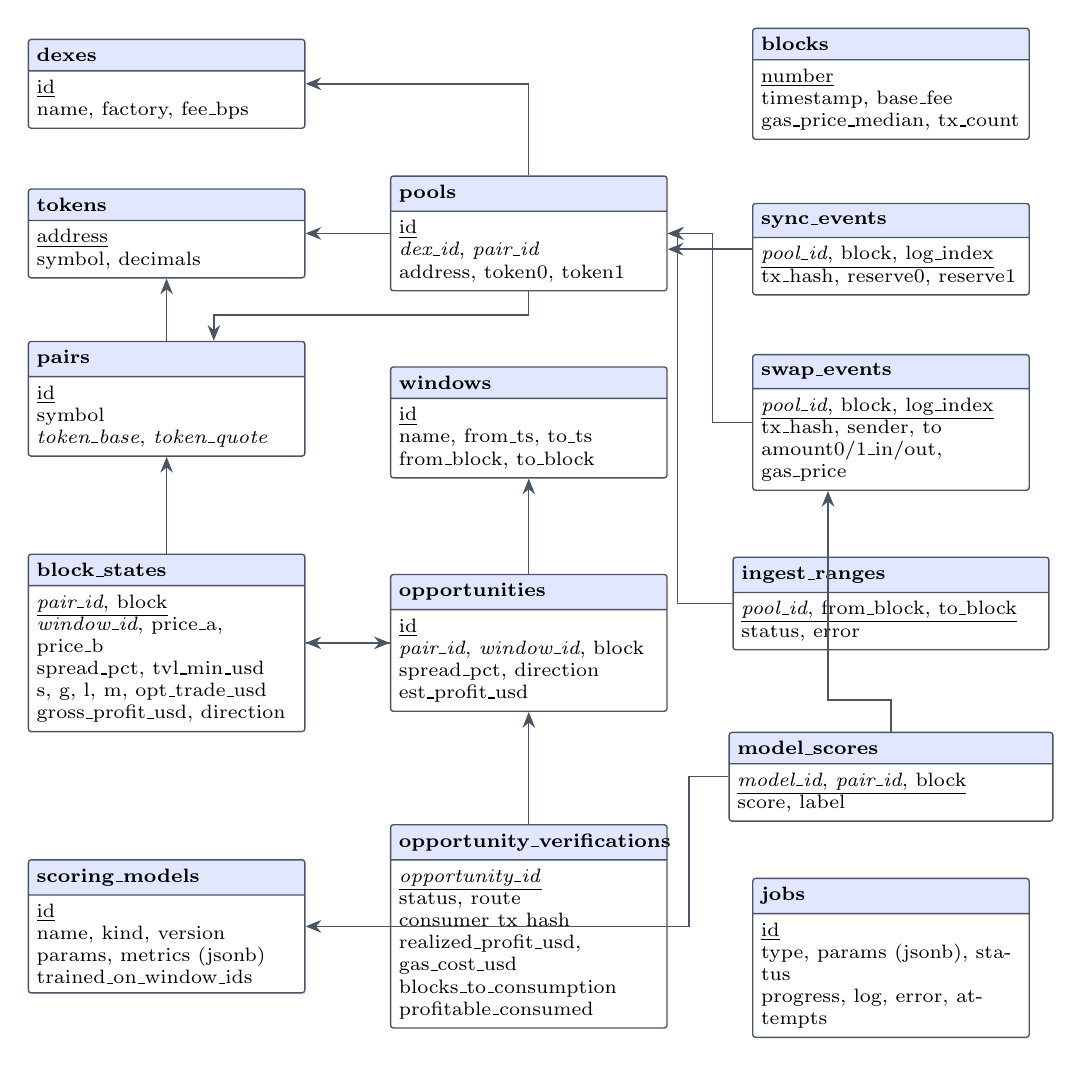
\begin{tikzpicture}[dg, x=1cm, y=1cm,
  ent/.style={draw=dgLine, rectangle split, rectangle split parts=2, rectangle split part fill={dgHead,white},
              align=left, inner sep=3pt, text width=33mm, font=\scriptsize, rounded corners=1pt},
  rel/.style={->, draw=dgLine, line width=.5pt}]
% kolumna 1: konfiguracja / pochodne
\node[ent] (dexes)  at (0,4.6)  {\textbf{dexes}\nodepart{second}\underline{id}\\name, factory, fee\_bps};
\node[ent] (tokens) at (0,2.7)  {\textbf{tokens}\nodepart{second}\underline{address}\\symbol, decimals};
\node[ent] (pairs)  at (0,0.6)  {\textbf{pairs}\nodepart{second}\underline{id}\\symbol\\\textit{token\_base}, \textit{token\_quote}};
\node[ent] (bs)     at (0,-2.5) {\textbf{block\_states}\nodepart{second}\underline{\textit{pair\_id}, block}\\\textit{window\_id}, price\_a, price\_b\\spread\_pct, tvl\_min\_usd\\s, g, l, m, opt\_trade\_usd\\gross\_profit\_usd, direction};
\node[ent] (models) at (0,-6.1) {\textbf{scoring\_models}\nodepart{second}\underline{id}\\name, kind, version\\params, metrics (jsonb)\\trained\_on\_window\_ids};
% kolumna 2
\node[ent] (pools)   at (4.6,2.7)  {\textbf{pools}\nodepart{second}\underline{id}\\\textit{dex\_id}, \textit{pair\_id}\\address, token0, token1};
\node[ent] (windows) at (4.6,0.3)  {\textbf{windows}\nodepart{second}\underline{id}\\name, from\_ts, to\_ts\\from\_block, to\_block};
\node[ent] (opp)     at (4.6,-2.5) {\textbf{opportunities}\nodepart{second}\underline{id}\\\textit{pair\_id}, \textit{window\_id}, block\\spread\_pct, direction\\est\_profit\_usd};
\node[ent] (ver)     at (4.6,-6.1) {\textbf{opportunity\_verifications}\nodepart{second}\underline{\textit{opportunity\_id}}\\status, route\\consumer\_tx\_hash\\realized\_profit\_usd, gas\_cost\_usd\\blocks\_to\_consumption\\profitable\_consumed};
% kolumna 3: surowe / oceny / kolejka
\node[ent] (blocks) at (9.2,4.6)  {\textbf{blocks}\nodepart{second}\underline{number}\\timestamp, base\_fee\\gas\_price\_median, tx\_count};
\node[ent] (sync)   at (9.2,2.5)  {\textbf{sync\_events}\nodepart{second}\underline{\textit{pool\_id}, block, log\_index}\\tx\_hash, reserve0, reserve1};
\node[ent] (swap)   at (9.2,0.3)  {\textbf{swap\_events}\nodepart{second}\underline{\textit{pool\_id}, block, log\_index}\\tx\_hash, sender, to\\amount0/1\_in/out, gas\_price};
\node[ent, text width=38mm] (ranges) at (9.2,-2.0) {\textbf{ingest\_ranges}\nodepart{second}\underline{\textit{pool\_id}, from\_block, to\_block}\\status, error};
\node[ent, text width=39mm] (scores) at (9.2,-4.2) {\textbf{model\_scores}\nodepart{second}\underline{\textit{model\_id}, \textit{pair\_id}, block}\\score, label};
\node[ent] (jobs)   at (9.2,-6.5) {\textbf{jobs}\nodepart{second}\underline{id}\\type, params (jsonb), status\\progress, log, error, attempts};

\draw[rel] (pools.north) |- (dexes.east);
\draw[rel] (pools.west) -- (tokens.east |- pools.west);
\draw[rel] (pools.south) -- ++(0,-.3) -| ([xshift=6mm]pairs.north);
\draw[rel] (pairs.north) -- (tokens.south);
\draw[rel] (sync.west) -- (pools.east |- sync.west);
\draw[rel] (swap.west) -- ++(-.5,0) |- (pools.east);
\draw[rel] (ranges.west) -- ++(-.7,0) |- (pools.east);
\draw[rel] (bs.north) -- (pairs.south);
\draw[rel] (bs.east) -- (windows.west |- bs.east);
\draw[rel] (opp.north) -- (windows.south);
\draw[rel] (opp.west) -- (bs.east |- opp.west);
\draw[rel] (ver.north) -- (opp.south);
\draw[rel] (scores.west) -- ++(-.5,0) |- (models.east);
\draw[rel] (scores.north) -- ++(0,.4) -| ([xshift=-8mm]swap.south);
\end{tikzpicture}
}
\caption{Schemat bazy danych; klucze główne podkreślone, obce kursywą (opracowanie własne)}\label{fig:erd}\end{figure}

\subsection{Pozyskiwanie danych z~łańcucha}

Jedynym źródłem danych jest węzeł archiwalny Ethereum odpytywany przez JSON-RPC. Rozważany wcześniej
import z~pliku CSV odrzucono po wykryciu uszkodzenia pola \texttt{logIndex} (ADR~0001).
Zadanie \texttt{ingest:pool-window} dla puli i~okna przebiega w~czterech krokach:
\begin{enumerate}[nosep]
  \item wyznacza (raz) zakres bloków okna przez wyszukiwanie binarne po znacznikach czasu
        i~zapisuje go w~\texttt{windows};
  \item dzieli zakres na porcje po \texttt{LOGS\_CHUNK\_BLOCKS} $=10\,000$ bloków; każda porcja jest
        wierszem \texttt{ingest\_ranges}, a~porcje ukończone są pomijane przy wznowieniu;
  \item dla każdej porcji wywołuje \texttt{eth\_getLogs} z~adresem puli i~jednym filtrem na dwa
        tematy (\texttt{Sync}, \texttt{Swap}); gdy węzeł odrzuca odpowiedź jako zbyt dużą, zakres
        jest rekurencyjnie dzielony na pół; logi są walidowane (adres, zakres), deduplikowane po
        \texttt{(block, logIndex)} i~dekodowane;
  \item dla bloków ze zdarzeniami pobiera \texttt{eth\_getBlockByNumber} z~pełnymi transakcjami
        w~pakietach JSON-RPC po 20 bloków, z~równoległością \texttt{RPC\_CONCURRENCY} $=4$,
        i~zapisuje znacznik czasu, \texttt{baseFee} oraz medianę efektywnej ceny gazu wszystkich
        transakcji bloku.
\end{enumerate}
Efektywna cena gazu transakcji jest liczona jednolicie dla obu modeli opłat z~rozdziału~2.1.
Dla transakcji typu~2 (po EIP-1559) wynosi $\min(\texttt{maxFeePerGas},\ \texttt{baseFee} +
\texttt{maxPriorityFeePerGas})$, w~pozostałych przypadkach jest równa \texttt{gasPrice}. Klient
RPC pracuje na liście adresów (węzeł własny, potem publiczne węzły zapasowe). Ponawia wywołanie
do sześciu razy z~wykładniczym odstępem od 1 do 30~s i~losowym rozrzutem, od drugiej nieudanej
próby rotując adres. Ponawiane są tylko błędy przejściowe: HTTP~429 i~5xx, błędy sieci
i~wybrane kody JSON-RPC.

\subsection{Wykrywanie okazji i~cechy $S$, $G$, $L$, $M$}

\paragraph{Stan pary w~bloku.} Zadanie \texttt{analyze:pair-window} odtwarza stan obu puli po
każdym bloku okna. Stanem puli jest zdarzenie \texttt{Sync} o~najwyższym \texttt{logIndex}
w~bloku; blok bez zdarzeń dziedziczy stan poprzedni. Rezerwy \texttt{reserve0/1} są orientowane
na rezerwę bazową i~kwotowaną przez porównanie adresów tokenów puli z~definicją pary. Kontrakt
sortuje tokeny po adresie, więc dla WETH/USDT token bazowy jest \texttt{token0}, a~dla
pozostałych par \texttt{token1}. Cena to kwotowany za jeden bazowy według wzoru~\eqref{eq:spot}
z~uwzględnieniem liczby miejsc dziesiętnych obu tokenów. Kurs ETH/USD do wyceny w~dolarach
pochodzi z~samej pary, gdy jest kwotowana w~stablecoinie; dla WBTC/WETH pochodzi z~pary
referencyjnej WETH/USDC w~tym samym bloku i~z~tego powodu planer analizuje WETH/USDC jako
pierwszą w~oknie.

\paragraph{Okazja i~optymalna transakcja.} Blok jest okazją, gdy rozbieżność~\eqref{eq:spread}
przekracza \texttt{SPREAD\_THRESHOLD\_PCT} $=0{,}65\,\%$, czyli sumę prowizji obu wymian
z~niewielkim marginesem (ADR~0002). Kierunek arbitrażu wyznacza porównanie cen mnożeniem
krzyżowym rezerw, bez dzielenia. Niech pula tańsza $A$ ma rezerwy $X_A$ tokena bazowego i~$Y_A$
kwotowanego, a~pula droższa $B$ odpowiednio $X_B$ i~$Y_B$. Zysk brutto z~wymiany $\Delta y$
jednostek tokena kwotowanego w~$A$ na token bazowy i~jego sprzedaży w~$B$ wynosi
$\Pi(\Delta y) = \mathrm{out}_B(\mathrm{out}_A(\Delta y)) - \Delta y$, gdzie $\mathrm{out}$ jest
funkcją~\eqref{eq:amountout}. Warunek $\Pi'(\Delta y)=0$ ma rozwiązanie zamknięte
\begin{equation}
  \Delta y^{*} = \frac{\gamma\sqrt{X_A Y_A X_B Y_B} - X_B Y_A}{\gamma\,(X_B + \gamma X_A)},
  \qquad \gamma = 1-\varphi ,
  \label{eq:opttrade}
\end{equation}
a~$\Delta y^{*}\le 0$ oznacza, że rozbieżność nie pokrywa dwóch prowizji. Implementacja
(fragment~\ref{lst:opttrade}) liczy~\eqref{eq:opttrade} w~arytmetyce całkowitej na
\texttt{bigint}, z~pierwiastkiem całkowitym metodą Newtona, tak jak liczy kontrakt. Zysk brutto
oblicza dwoma wywołaniami \texttt{getAmountOut}. Oba wyniki są wyceniane w~USD jako
\texttt{gross\_profit\_usd} i~\texttt{opt\_trade\_usd}.

\lstinputlisting[language=TypeScript,
  caption={Optymalna wielkość transakcji i~zysk brutto (\texttt{packages/core/src/amm.ts}, l.~50--79)},
  label={lst:opttrade}]{Listings/opt-trade.ts}

\paragraph{Cechy.} Dla każdego bloku obliczane są cztery cechy wejściowe modelu FIS
(tab.~\ref{tab:features}). Cecha $G$ odnosi koszt gazu transakcji arbitrażowej
(\texttt{ARB\_GAS} $=220\,000$ jednostek: dwie wymiany i~transfer) do transakcji referencyjnej
o~wartości \texttt{REF\_TRADE\_USD} $=50\,000$~USD. Cecha $M$ jest indeksem ryzyka konkurencji:
średnią rang percentylowych liczby swapów w~bloku (aktywność botów) i~ceny gazu, liczonych
w~obrębie całego okna. Cena gazu bloków bez własnych zdarzeń jest interpolowana liniowo między
sąsiednimi blokami ze zdarzeniami analizowanej pary. Obcięcie do dziedzin zmiennych rozmytych
odbywa się w~jednym miejscu (\texttt{computeRawFeatures}); modele dostają wartości już obcięte.

\begin{table}[H]\centering\small
\caption{Cechy opisujące okazję w~bloku}\label{tab:features}
\begin{tabular}{llll}
\toprule
Cecha & Wzór & Jednostka & Dziedzina \\
\midrule
$S$ & $|p_A-p_B|/\min(p_A,p_B)\cdot 100$ & \% & $[0,3]$ \\
$G$ & $\texttt{ARB\_GAS}\cdot g_{\mathrm{gwei}}\cdot 10^{-9}\cdot \mathrm{ETHUSD}\,/\,\texttt{REF\_TRADE\_USD}\cdot 100$ & \% wartości tx & $[0,2]$ \\
$L$ & $\min(\mathrm{TVL}_A,\mathrm{TVL}_B)/10^{6}$, $\mathrm{TVL}=2\cdot Y\cdot \mathrm{quoteUSD}$ & mln USD & $[0,100]$ \\
$M$ & $100\cdot\big(0{,}5\cdot\mathrm{pctl}(\text{swapy w~bloku}) + 0{,}5\cdot\mathrm{pctl}(g_{\mathrm{gwei}})\big)$ & pkt & $[0,100]$ \\
\bottomrule
\end{tabular}
\end{table}

\subsection{Modele oceny wykonalności}

Cztery modele implementują wspólny interfejs \texttt{ScoringModel}: z~cech bloku zwracają ocenę
$\mathrm{score}\in[0,100]$ oraz etykietę. Wspólny próg decyzyjny to $\mathrm{score}\ge 50$.
Próg ten (\texttt{SCORE\_THRESHOLD}) służy wyłącznie klasyfikacji binarnej w~ewaluacji: blok jest
przewidywany jako wykonalny, gdy $\mathrm{score}\ge 50$. Etykieta słowna jest od niego niezależna
i~w~modelach rozmytych wynika z~funkcji przynależności termów $W$ (p.~3.6.2), więc ocena
z~przedziału $[50;\,52{,}5)$ liczy się jako pozytywna, choć nosi jeszcze etykietę ,,ryzykowna''.

\subsubsection{Heurystyka progowa (baseline~v1)}
Zysk netto wynosi $\mathrm{net} = \mathrm{gross} - \texttt{ARB\_GAS}\cdot g\cdot\mathrm{ETHUSD}$.
Okazja jest wykonalna, gdy $\Delta y^{*}>0$ i~$\mathrm{net}>0$. Ocena to
$\mathrm{clamp}(\mathrm{ROI}\cdot 10\,000,\,0,\,100)$ z~$\mathrm{ROI}=\mathrm{net}/\Delta y^{*}$,
więc ROI równe $1\,\%$ daje 100 punktów. Etykieta jest binarna. Model nie ma parametrów
strojonych i~stanowi punkt odniesienia.

\subsubsection{System wnioskowania rozmytego Mamdaniego}
Model zaimplementowano na bibliotece \texttt{@thi.ng/fuzzy}. Cztery
zmienne wejściowe mają po trzy termy, zmienna wyjściowa $W$ (wykonalność) cztery
(tab.~\ref{tab:terms}). Funkcje przynależności to rampy na krańcach dziedziny i~trójkąty
w~środku. Baza zawiera 16 reguł (fragment~\ref{lst:rules}; pełna lista w~załączniku~C). Reguły
R1--R4 mają konkluzję ,,niewykonalna'' i~zapisują warunki konieczne wykonalności (znikoma
rozbieżność; zaporowy gaz; umiarkowana rozbieżność przy płytkiej płynności; umiarkowana
rozbieżność przy umiarkowanym gazie i~ryzyku MEV innym niż niskie). Nie są one jednak wetem
w~ścisłym sensie: nie ma osobnego mechanizmu poza zwykłą agregacją, więc pozostałe odpalone reguły
też wchodzą do wyniku, a~pełna aktywacja reguły z~R1--R4 przesuwa ocenę ku dołowi skali, nie
wyłączając innych reguł. Operatory: AND $=\min$, implikacja $=\min$, agregacja $=\max$,
defuzyfikacja centroidem~\eqref{eq:centroid} na 500 próbkach.
Etykietą jest term wyjściowy o~najwyższej przynależności dla wartości po defuzyfikacji (funkcja
\texttt{labelForScore}, wspólna dla baseline~v2, systemu Mamdaniego i~ANFIS), więc granice etykiet wynikają z~przecięć
funkcji przynależności, nie z~okrągłych progów. Stopnie aktywacji reguł są zwracane razem
z~oceną i~pokazywane w~interfejsie jako wyjaśnienie.

\begin{table}[H]\centering\footnotesize
\caption{Termy zmiennych rozmytych; \texttt{iR}$(a,b)$ --- rampa opadająca,
  \texttt{tri}$(a,b,c)$ --- trójkąt, \texttt{R}$(a,b)$ --- rampa rosnąca}\label{tab:terms}
\begin{tabular}{llll}
\toprule
Zmienna & Term 1 & Term 2 & Term 3 \\
\midrule
$S$ [\%] & znikoma \texttt{iR}(0{,}3; 0{,}65) & umiarkowana \texttt{tri}(0{,}5; 0{,}9; 1{,}4) & duża \texttt{R}(1{,}1; 1{,}8) \\
$G$ [\%] & niski \texttt{iR}(0{,}1; 0{,}3) & umiarkowany \texttt{tri}(0{,}2; 0{,}45; 0{,}8) & zaporowy \texttt{R}(0{,}6; 1{,}0) \\
$L$ [mln USD] & płytka \texttt{iR}(2; 8) & średnia \texttt{tri}(5; 20; 45) & głęboka \texttt{R}(35; 60) \\
$M$ [pkt] & niskie \texttt{iR}(20; 40) & średnie \texttt{tri}(30; 50; 70) & wysokie \texttt{R}(60; 80) \\
\midrule
$W$ [pkt] & niewykonalna \texttt{iR}(15; 30) & ryzykowna \texttt{tri}(25; 40; 55) & wykonalna \texttt{tri}(50; 65; 80) \\
          &                                  &                                    & atrakcyjna \texttt{R}(75; 90) \\
\bottomrule
\end{tabular}
\end{table}

\lstinputlisting[language=TypeScript,
  caption={Baza reguł systemu Mamdaniego (\texttt{packages/core/src/mamdani.params.ts}, l.~115--135)},
  label={lst:rules}]{Listings/rules.ts}

\subsubsection{Heurystyka kalibrowana (baseline~v2)}
Analiza transakcji konsumujących wykazała, że boty zużywają medianowo ok.~153\,000 gazu, nie
220\,000, a~część z~nich płaci za gaz poza polem transakcji (pakiety Flashbots). Koszt z~modelu
v1 jest więc zawyżony. Baseline~v2 (ADR~0006) zachowuje deterministyczną postać, ale jego
parametry są dobierane na etykietach z~weryfikacji:
\begin{align}
  \mathrm{net}_2 &= \mathrm{gross} - \frac{\mathrm{gasUnits}}{220\,000}\cdot \kappa \cdot
  \mathrm{gasCost}_{v1}, \label{eq:bv2}\\
  v &= (1-w)\,\sigma\!\left(\frac{\mathrm{net}_2}{s}\right) + w\cdot \mathrm{rank}(\Delta y^{*}),
  \nonumber
\end{align}
W~równaniu~\eqref{eq:bv2} $\sigma$ jest funkcją logistyczną, $s=1{,}4826\cdot\mathrm{MAD}(\mathrm{net}_2)$ odpornym
rozrzutem na zbiorze kalibracyjnym, $\mathrm{rank}$ rangą decylową wielkości transakcji, a~$v=0$
dla $\mathrm{gross}\le 0$. Ocena jest odcinkowo-liniowym odwzorowaniem $v$, w~którym próg
F1-optymalny $t$ trafia na 50 punktów. Kalibracja przeszukuje siatkę $\mathrm{gasUnits}\in
\{150\,000, 220\,000\}\times\kappa\in\{0;0{,}25;0{,}5;0{,}75;1\}\times w\in\{0;0{,}25;0{,}5\}$
(30 kombinacji) i~wybiera punkt o~najwyższym AUC, przy remisie o~wyższym $F_1$. Procedura nie
zawiera losowości.

\subsubsection{ANFIS}
Model Takagiego--Sugeno pierwszego rzędu o~strukturze pięciowarstwowej (rozdział~2.4) z~tą samą
bazą 16 reguł, co system Mamdaniego. Przesłanki są funkcjami Gaussa z~plateau (trzy na zmienną,
12 termów), inicjalizowanymi z~termów Mamdaniego przy zachowaniu środka i~szerokości połówkowej.
Klauzule negowane współdzielą parametry z~termem bazowym i~liczą $1-\mu$. Siła reguły to
iloczyn przynależności, różniczkowalny w~odróżnieniu od minimum. Konkluzje $f_i = p_i S' + q_i
G' + r_i L' + s_i M' + t_i$ działają na cechach standaryzowanych statystykami zbioru treningowego,
a~wyjście $y=\sigma(\sum_i \bar w_i f_i)$ daje $\mathrm{score}=100\,y$. Konkluzje startowe
$t_i=\mathrm{logit}(c_i/100)$ z~$c_i\in\{15,40,65,90\}$, środkiem termu wyjściowego reguły,
sprawiają, że model przed treningiem zachowuje się podobnie do systemu Mamdaniego.

Wszystkie parametry, przesłanki i~konkluzje, optymalizuje Adam ($\beta_1=0{,}9$,
$\beta_2=0{,}999$, $\mathrm{lr}=0{,}01$, minipaczki 256) na ważonej binarnej entropii krzyżowej
z~wagą klasy pozytywnej $\min(N_-/N_+,\,50)$. Trening trwa najwyżej 200 epok, z~wczesnym
zatrzymaniem po 10 epokach bez poprawy straty walidacyjnej na 20\,\% grup. Po każdym kroku
szerokości $\sigma$ są ograniczane od dołu do $1\,\%$ szerokości dziedziny. Cały stan losowy
(podział, tasowanie) pochodzi z~jednego generatora o~zadanym ziarnie, więc trening jest
odtwarzalny co do bitu. Zbiór uczący tworzą wszystkie zweryfikowane okazje o~znanej etykiecie
oraz tło (bloki bez okazji) podpróbkowane w~stosunku $10:1$ do liczby pozytywów. Okazje
o~trasie \texttt{multi} są pomijane jako nieoznaczone (rozdział~3.7).

\subsection{Weryfikacja retrospektywna okazji}

Etykietę ,,okazja była wykonalna'' system wyznacza z~faktów on-chain (rys.~\ref{fig:verify}). Dla
okazji z~bloku $B$ zadanie \texttt{verify:pair-window} obserwuje bloki $B\ldots B+K_{\max}$,
$K_{\max}=3$, i~przypisuje jeden z~czterech statusów:
\begin{itemize}[nosep]
  \item \texttt{consumed\_atomic}: w~oknie istnieje transakcja zawierająca \texttt{Swap} w~obu
        pulach pary o~przeciwnych kierunkach (kupno bazowego w~jednej, sprzedaż w~drugiej); brana
        jest pierwsza taka transakcja według \texttt{(block, logIndex)}, a~jej paragon musi mieć
        \texttt{status = 1};
  \item \texttt{consumed\_partial}: brak transakcji atomowej, ale w~pierwszym bloku $B+k$,
        w~którym rozbieżność spadła poniżej progu, istnieje swap ją zawężający (sprzedaż w~puli
        droższej lub kupno w~tańszej);
  \item \texttt{decayed}: rozbieżność spadła poniżej progu bez identyfikowalnej transakcji;
  \item \texttt{persisted}: rozbieżność utrzymała się we wszystkich obserwowanych blokach.
\end{itemize}
Warunek ,,swap w~tym samym bloku'' dla statusu częściowego jest celowy. Dopuszczenie
wcześniejszych bloków wiązało okazję z~niepowiązanymi transakcjami.

Dla konsumpcji atomowej pobierany jest paragon (\texttt{eth\_getTransactionReceipt}, pakiety po 20)
i~dekodowane są zdarzenia \texttt{Transfer} obu tokenów pary. Zawinięcie i~odwinięcie WETH nie
emituje \texttt{Transfer}, dlatego zdarzenia \texttt{Deposit}/\texttt{Withdrawal} kontraktu WETH są
zamieniane na syntetyczne przepływy przypisane zawsze nadawcy transakcji (ADR~0004: ETH
$\equiv$ WETH). Bez tej korekty router odwijający WETH wyglądał na beneficjenta całej kwoty.
Beneficjentem jest adres o~maksymalnym netto USD przepływów tokenów pary spośród kandydatów
(odbiorcy obu swapów, nadawca i~adresat transakcji, odbiorcy transferów; pule są wykluczone),
a~remisy rozstrzyga kolejność: adresat, potem nadawca (ADR~0005). Wcześniejsza, prostsza
heurystyka zaniżała zysk do zera dla ok.~62\,\% konsumpcji. Trasa transakcji jest klasyfikowana
jako \texttt{two\_pool}, gdy paragon zawiera wyłącznie swapy obu puli pary i~transfery jej tokenów
(oraz WETH); w~przeciwnym razie jako \texttt{multi} (ADR~0003). Okazja o~trasie \texttt{multi}
nadal była skonsumowana, ale zysk konsumenta jest nieznany, więc wiersz jest wykluczony
z~populacji uczenia i~ewaluacji, co wymusza \texttt{CHECK} w~bazie. Ostatecznie
\begin{equation}
  \begin{split}
  \texttt{profitable\_consumed} \Leftrightarrow{}&
  \text{status}=\texttt{consumed\_atomic} \wedge \text{route}=\texttt{two\_pool}\\
  &\wedge\ \mathrm{profit}_{\mathrm{real}} - \mathrm{gasCost} > 0,
  \end{split}
  \label{eq:label}
\end{equation}
gdzie $\mathrm{gasCost} = \mathrm{gasUsed}\cdot\mathrm{effectiveGasPrice}\cdot\mathrm{ETHUSD}$.
Etykieta~\eqref{eq:label} jest zmienną celu w~kalibracji i~uczeniu modeli. Rdzeń klasyfikacji pokazuje fragment~\ref{lst:classify}. Heurystyki sprawdzono ręcznie na próbie
transakcji (rozdział~4.3).

\lstinputlisting[language=TypeScript,
  caption={Klasyfikacja statusu okazji (\texttt{packages/analysis/src/verify/classify.ts}, l.~81--133)},
  label={lst:classify}]{Listings/classify.ts}

\begin{figure}[H]\centering\resizebox{\linewidth}{!}{% Diagram sekwencji weryfikacji retrospektywnej
\begin{tikzpicture}[dg, x=1cm, y=1cm,
  life/.style={box, minimum width=28mm, minimum height=9mm},
  act/.style={draw=dgLine, fill=dgHead, minimum width=2.4mm, inner sep=0pt, anchor=north},
  msg/.style={->, draw=dgLine, line width=.6pt},
  ret/.style={->, draw=dgLine, line width=.6pt, dashed},
  ml/.style={font=\scriptsize, above, inner sep=1.5pt},
  stp/.style={font=\scriptsize\itshape, text=dgLine, anchor=west, inner sep=2pt}]
\def\H{-9.2}
\node[life] (w)   at (0,0)    {\texttt{worker}};
\node[life] (v)   at (4.6,0)  {\texttt{analysis/verify}};
\node[life] (db)  at (9.2,0)  {PostgreSQL};
\node[life] (rpc) at (13.8,0) {Węzeł RPC};
\foreach \n in {w,v,db,rpc} \draw[draw=dgLine!60, dash pattern=on 2pt off 2pt] (\n.south) -- ++(0,\H);

\node[act, minimum height=8.2cm] at (w |- 0,-.45) {};
\draw[msg] (w |- 0,-1.0) -- node[ml] {okazje (paczka 200)} (v |- 0,-1.0);
\node[act, minimum height=6.8cm] at (v |- 0,-1.0) {};

\draw[msg] (v |- 0,-1.8) -- node[ml] {swapy, spready $B\ldots B{+}3$} (db |- 0,-1.8);
\draw[ret] (db |- 0,-2.4) -- (v |- 0,-2.4);
\node[stp] at (4.8,-3.0) {1. wybór transakcji-kandydata};

\draw[msg] (v |- 0,-3.7) -- node[ml] {\texttt{eth\_getTransactionReceipt} (paczka 20)} (rpc |- 0,-3.7);
\draw[ret] (rpc |- 0,-4.3) -- node[ml] {paragony} (v |- 0,-4.3);
\node[stp] at (4.8,-4.9) {2. przepływy tokenów, beneficjent, trasa};
\node[stp] at (4.8,-5.4) {3. status, opóźnienie $k$, zysk, koszt gazu};

\draw[msg] (v |- 0,-6.2) -- node[ml] {zapis weryfikacji} (db |- 0,-6.2);
\draw[ret] (v |- 0,-7.0) -- node[ml] {gotowe} (w |- 0,-7.0);
\draw[msg] (w |- 0,-7.8) -- node[ml] {postęp zadania} (db |- 0,-7.8);
\end{tikzpicture}
}
\caption{Przebieg weryfikacji retrospektywnej okazji (opracowanie własne)}\label{fig:verify}\end{figure}

\subsection{Kolejka zadań i~interfejs programistyczny}

Kolejka zadań jest tabelą \texttt{jobs} w~PostgreSQL. Proces \texttt{worker} pobiera najstarsze
zadanie w~stanie \texttt{queued} zapytaniem z~\texttt{FOR UPDATE SKIP LOCKED}, więc równoległe
procesy nie podjęłyby tego samego zadania. Częściowy indeks unikalny na \texttt{(type, params)}
dla zadań aktywnych zapobiega zdublowaniu zlecenia. Zadanie raportuje do bazy postęp (0--100)
i~dziennik. Po błędzie przejściowym wraca do kolejki z~wykładniczym odstępem, do
\texttt{JOB\_MAX\_ATTEMPTS} $=3$ prób; zadania przerwane restartem procesu są przywracane bez
zużycia próby. Sześć typów zadań tworzy łańcuch \texttt{ingest:pool-window} $\rightarrow$
\texttt{analyze:pair-window} $\rightarrow$ \texttt{verify:pair-window} $\rightarrow$
\texttt{calibrate:baseline\_v2} / \texttt{train}. Planer macierzy generuje ten łańcuch dla
czterech par i~czterech okien, łącznie 64 zadania danych.

Serwer API (Fastify) udostępnia 16 punktów końcowych (pełna lista --- załącznik~E): katalog (\texttt{/pairs},
\texttt{/windows}, \texttt{/models}), pokrycie danych, szeregi czasowe pary w~oknie z~agregacją
w~SQL, stronicowaną listę okazji z~filtrami (status, minimalna rozbieżność, model), szczegóły
okazji (cechy, rezerwy, aktywacje reguł, weryfikacja), ewaluację modelu na oknie, zlecanie
i~podgląd zadań, trening ANFIS, kalibrację baseline~v2 oraz migawkę trybu na żywo. Każda
odpowiedź jest walidowana schematem zod z~pakietu \texttt{shared} także po stronie serwera, co
gwarantuje zgodność kontraktu z~interfejsem. Serwer nie ma uwierzytelniania. Jest narzędziem
lokalnym i~to ograniczenie opisano w~rozdziale~4.8.

\subsection{Interfejs użytkownika}

Interfejs (React, Vite) ma pięć widoków. \emph{Dane} to siatka pokrycia par i~okien
z~przyciskami zlecania zadań oraz lista zadań z~postępem (rys.~\ref{fig:ui-dane}). \emph{Okno} pokazuje cztery wykresy dla
pary w~oknie (ceny obu puli, rozbieżność z~progiem, cena gazu, oceny modeli) ze wspólnym
zakresem bloków sterowanym suwakiem (rys.~\ref{fig:ui-okno}). \emph{Okazje} to stronicowana tabela z~filtrami
utrwalanymi w~adresie URL i~panel szczegółów okazji, w~tym aktywacje reguł Mamdaniego
i~odnośnik do Etherscan (rys.~\ref{fig:ui-okazje}; sam panel --- rys.~\ref{fig:ui-okazja}). \emph{Modele} zestawia modele: macierze pomyłek, nałożone krzywe ROC,
histogramy ocen, tabelę metryk oraz formularze treningu i~kalibracji (rys.~\ref{fig:ui-modele}). \emph{Na żywo} prezentuje
bieżący stan ośmiu puli próbkowany co 15~s (\texttt{eth\_call getReserves} i~logi swapów
z~ostatnich 20 bloków), oceniany tymi samymi modelami, z~historią ostatniej godziny w~pamięci
procesu API (rys.~\ref{fig:ui-live}). Dane odświeża odpytywanie (TanStack Query), bez
WebSocketów.
\begin{figure}[H]\centering
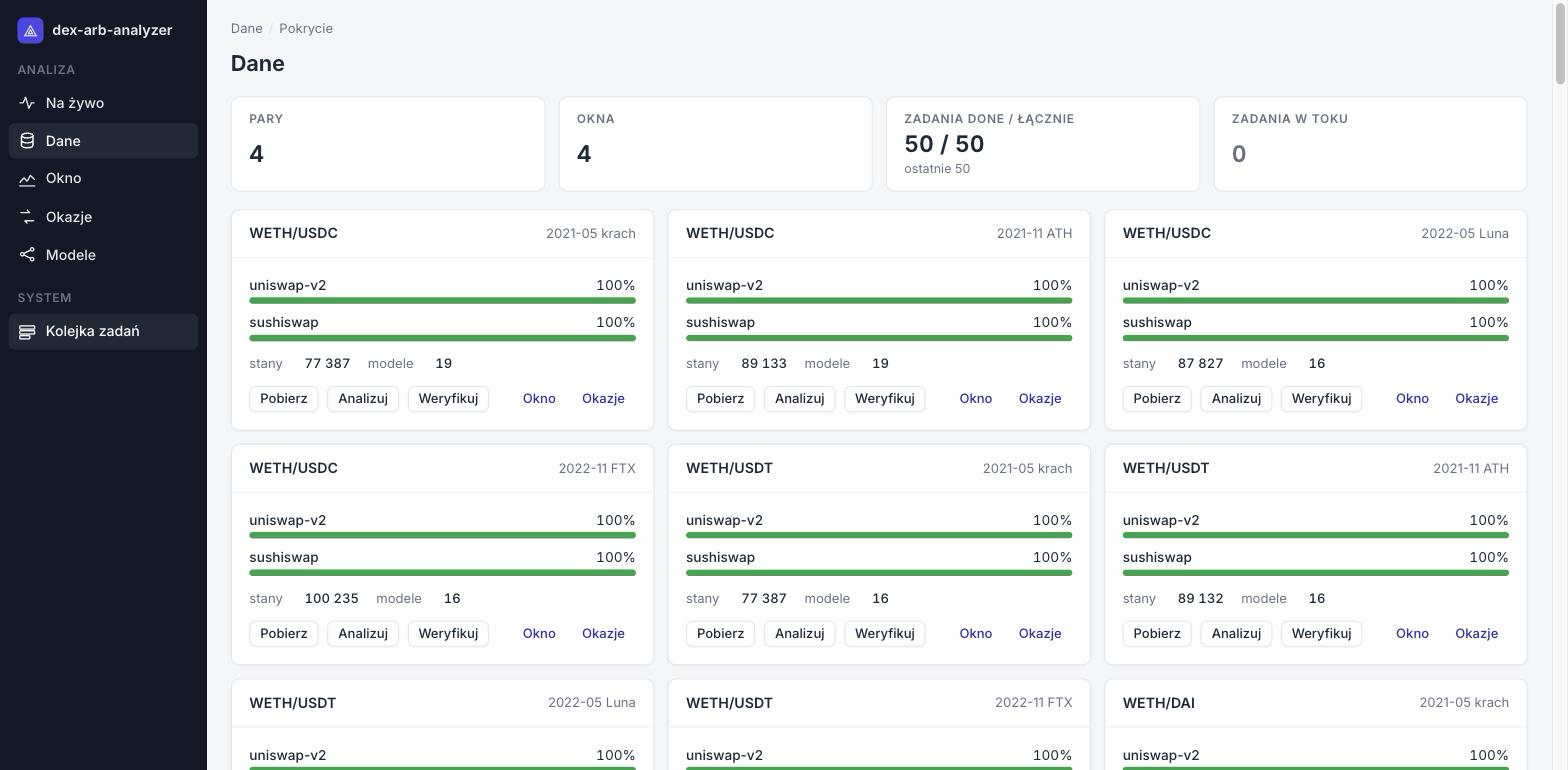
\includegraphics[width=\linewidth]{Images/ui-dane.png}
\caption{Widok \emph{Dane}: pokrycie par i~okien danymi obu pul oraz stan kolejki zadań
(zrzut ekranu, fragment)}\label{fig:ui-dane}
\end{figure}
\begin{figure}[H]\centering
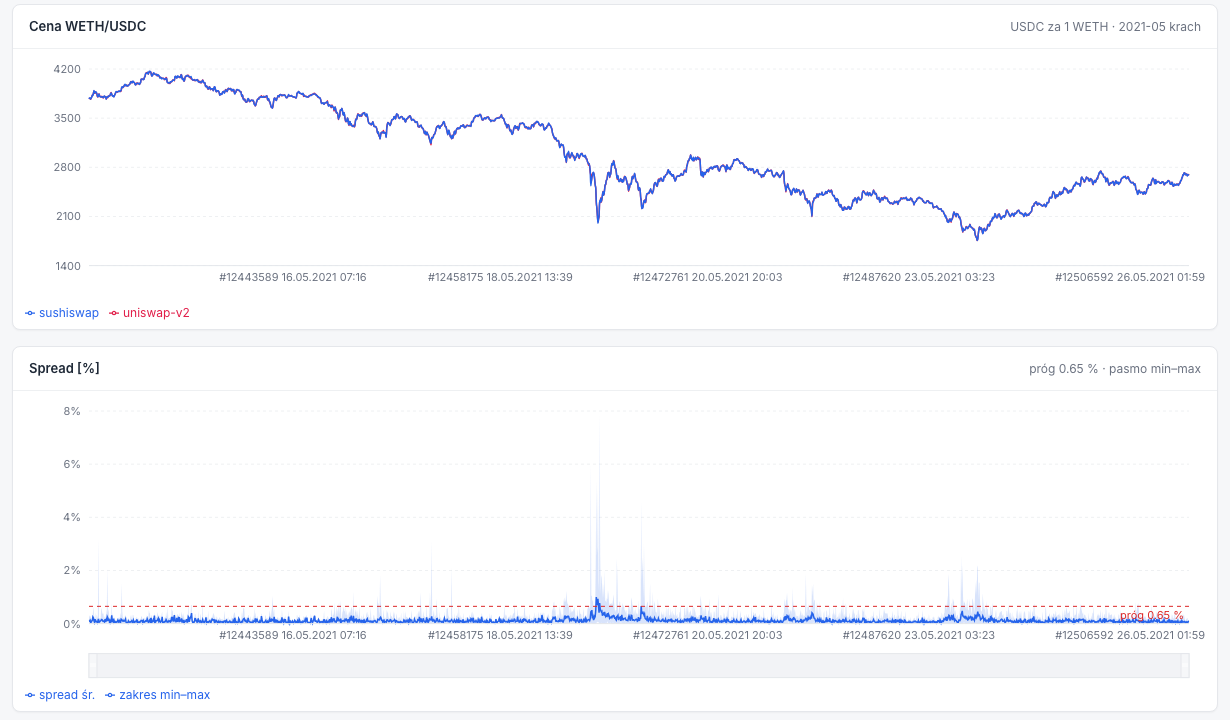
\includegraphics[width=.84\linewidth]{Images/ui-okno.png}
\caption{Widok \emph{Okno}: ceny obu puli i~rozbieżność z~progiem (WETH/USDC, okno 2021-05; zrzut ekranu, fragment)}\label{fig:ui-okno}
\end{figure}
\begin{figure}[H]\centering
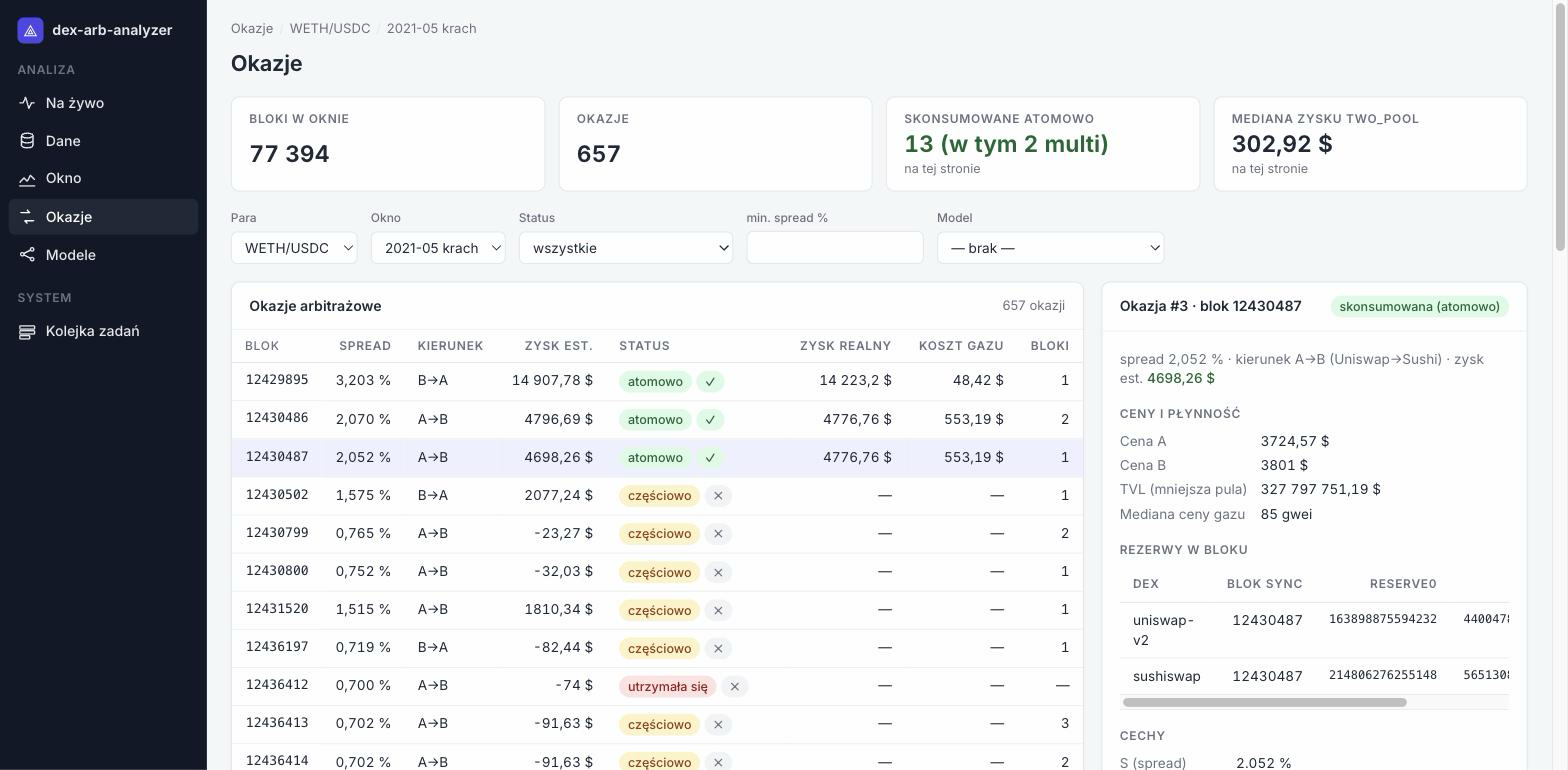
\includegraphics[width=\linewidth]{Images/ui-okazje.png}
\caption{Widok \emph{Okazje}: lista okazji w~oknie z~filtrami, statusem weryfikacji
i~zyskiem zrealizowanym (WETH/USDC, okno 2021-05; zrzut ekranu, fragment)}\label{fig:ui-okazje}
\end{figure}
\begin{figure}[H]\centering
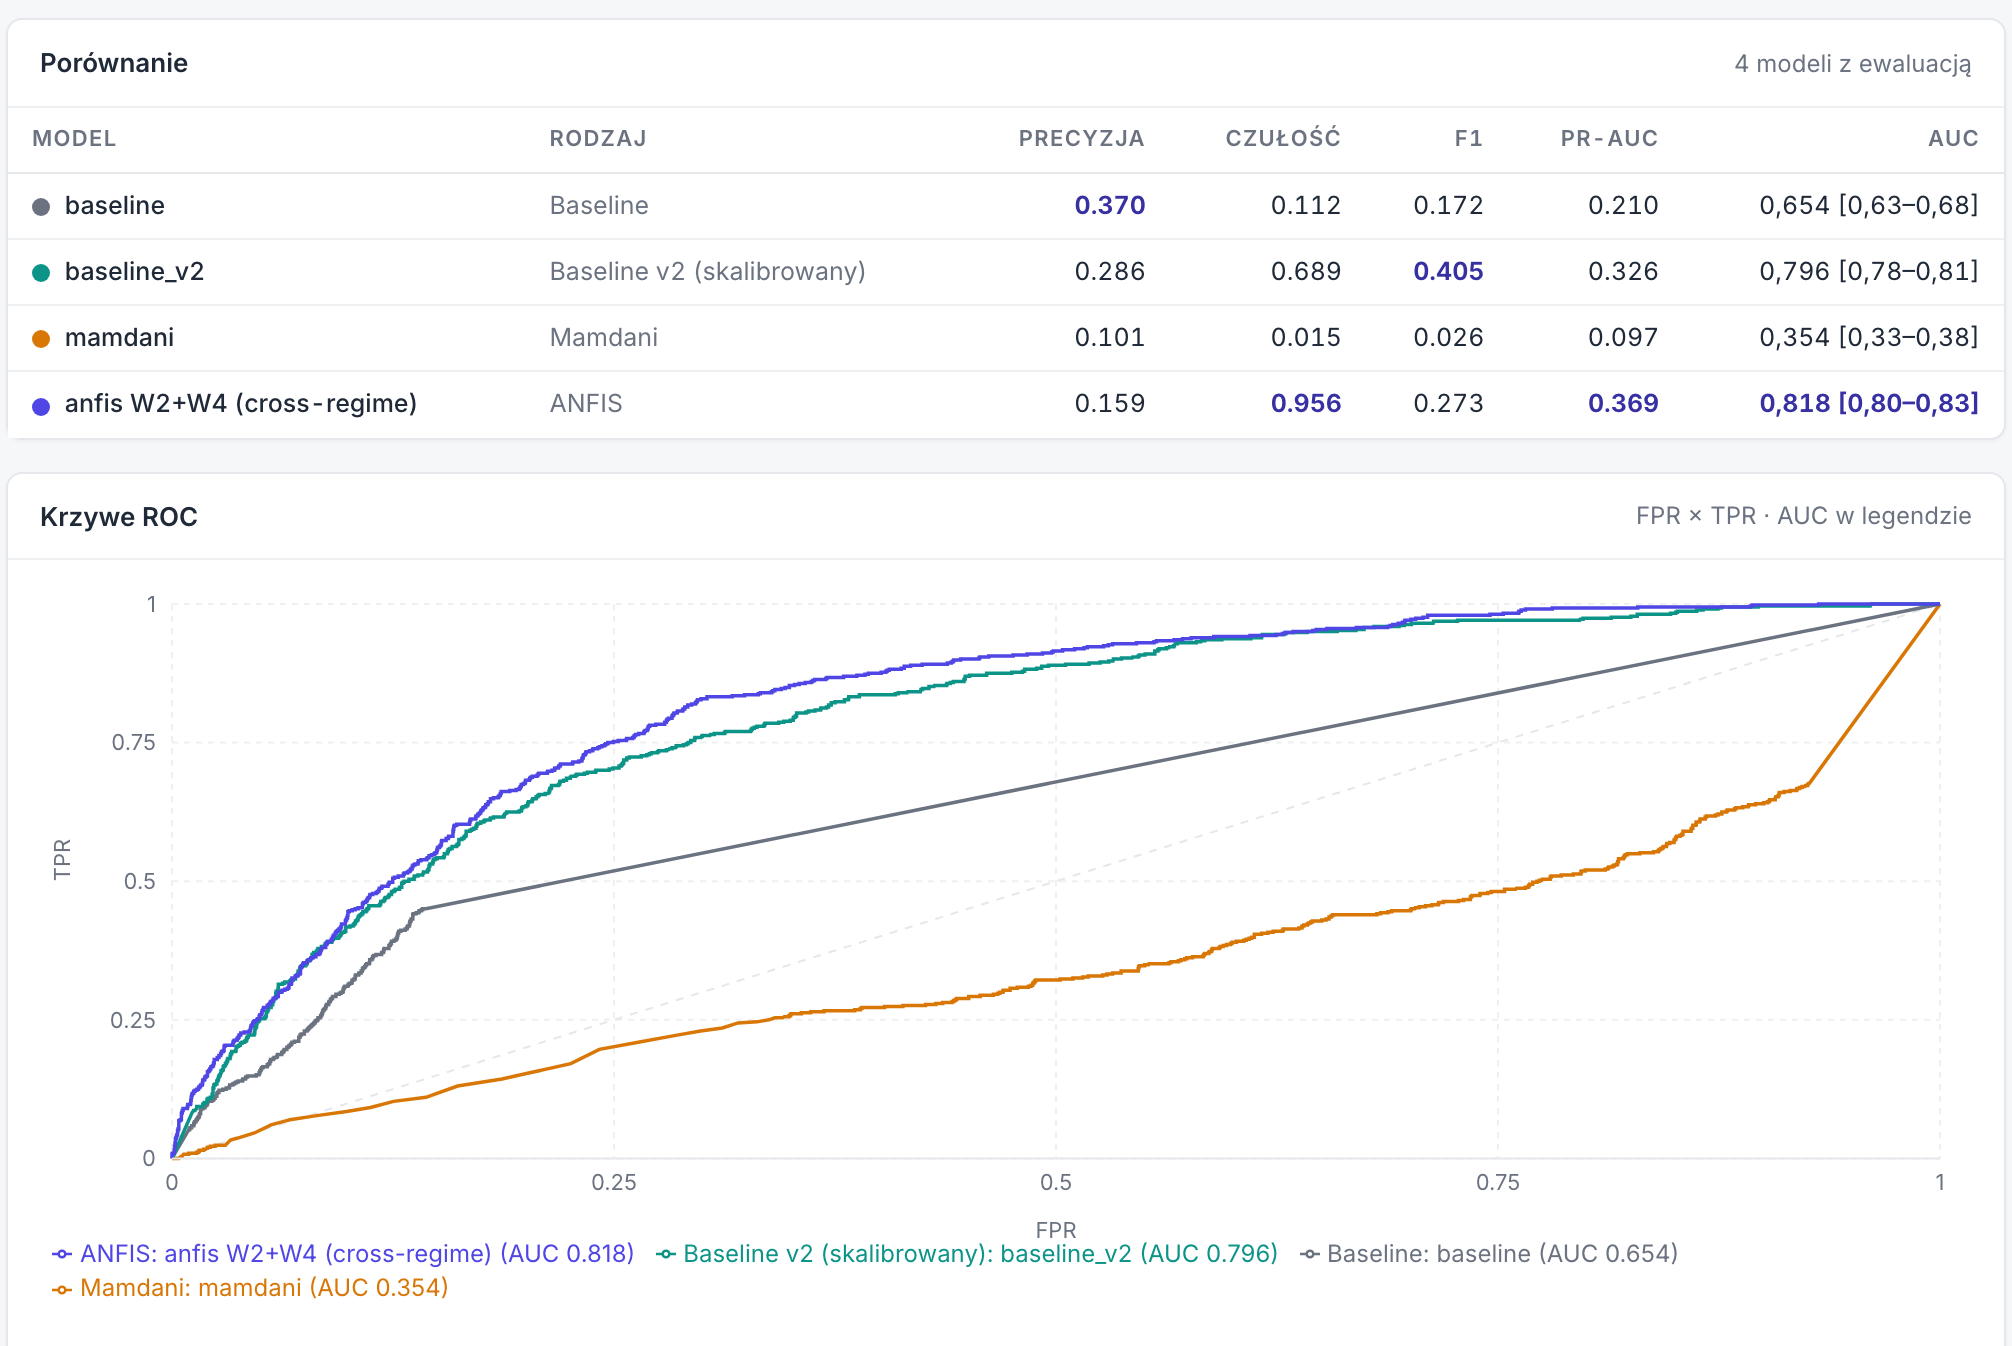
\includegraphics[width=\linewidth]{Images/ui-modele.png}
\caption{Widok \emph{Modele}: tabela metryk i~krzywe ROC czterech modeli na wszystkich oknach (zrzut ekranu, fragment)}\label{fig:ui-modele}
\end{figure}
\begin{figure}[H]\centering
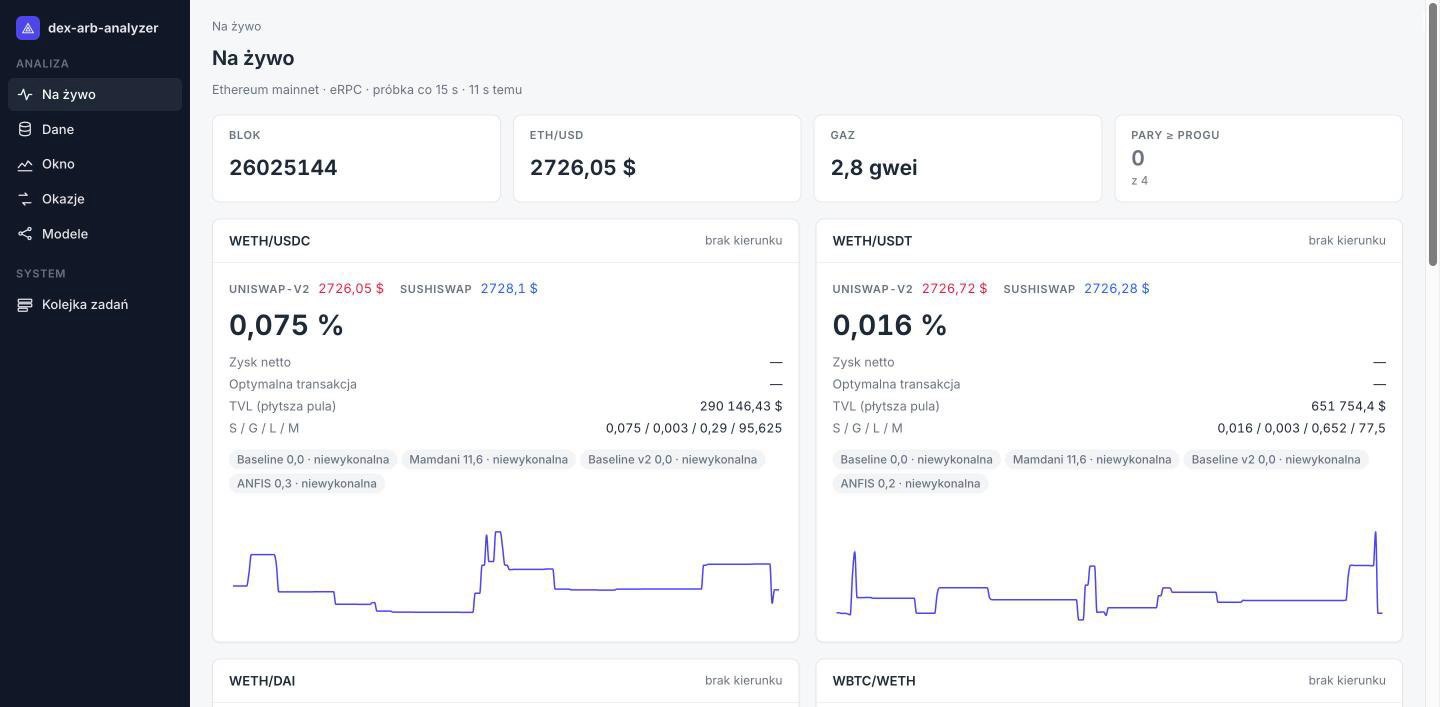
\includegraphics[width=\linewidth]{Images/ui-live.png}
\caption{Widok \emph{Na żywo}: bieżąca rozbieżność cen obu puli, cechy $S/G/L/M$ i~oceny
czterech modeli dla par próbkowanych co 15~s (zrzut ekranu, fragment)}\label{fig:ui-live}
\end{figure}

\newpage
\section{Badania i~wyniki}

\subsection{Zbiór danych}

Badania przeprowadzono na czterech parach tokenów (WETH/USDC, WETH/USDT, WETH/DAI, WBTC/WETH), po
jednej puli na każdej z~dwóch giełd, w~czterech dwutygodniowych oknach obejmujących okresy
gwałtownych ruchów cen (tab.~\ref{tab:windows}). Pokrycie danymi każdej z~32 kombinacji pula--okno
wynosi 100\,\% bloków okna (\texttt{results/coverage.csv}). Łącznie baza zawiera 250\,373 bloki
z~metadanymi, 795\,618 zdarzeń \texttt{Sync}, 786\,828 zdarzeń \texttt{Swap} i~1\,418\,144 stany
par w~blokach. Rozbieżność powyżej progu $0{,}65\,\%$ wystąpiła w~4\,829 blokach, co stanowi
$0{,}34\,\%$ wszystkich stanów; wszystkie te okazje poddano weryfikacji retrospektywnej.

\begin{table}[H]\centering\small
\caption{Okna analizy i~liczności (cztery pary łącznie)}\label{tab:windows}
\begin{tabular}{llrrrr}
\toprule
Okno & Daty (UTC) & Bloki & Stany par & Okazje & Okazje/stany \\
\midrule
2021-05 krach & 14--26.05.2021 & 12\,429\,199--12\,506\,592 & 309\,548 & 2\,236 & 0{,}72\,\% \\
2021-11 ATH   & 05--19.11.2021 & 13\,553\,257--13\,642\,393 & 356\,441 & 891   & 0{,}25\,\% \\
2022-05 Luna  & 05--19.05.2022 & 14\,713\,964--14\,801\,795 & 351\,295 & 1\,296 & 0{,}37\,\% \\
2022-11 FTX   & 05--19.11.2022 & 15\,900\,096--16\,000\,337 & 400\,860 & 406   & 0{,}10\,\% \\
\bottomrule
\end{tabular}
\end{table}

Wynik weryfikacji retrospektywnej zestawia tabela~\ref{tab:verif}. Status
\texttt{consumed\_atomic} otrzymało 714 okazji, z~czego 570 o~trasie \texttt{two\_pool}
i~144 o~trasie \texttt{multi} (wykluczone z~populacji ewaluacji). Etykietę pozytywną
(\texttt{profitable\_consumed}) ma 544 okazji, czyli $11{,}6\,\%$ populacji o~znanej etykiecie
($n=4\,685$). Udział konsumpcji atomowych jest najwyższy w~oknie 2021-05 (27,6\,\% okazji). W~trzech
późniejszych oknach wynosi już tylko 2,7--4,6\,\%, a~w~oknie 2022-11 dla par WETH/DAI
i~WBTC/WETH nie zarejestrowano ani jednej. Rozkład opóźnienia konsumpcji dla trasy
\texttt{two\_pool} przedstawia rys.~\ref{fig:khist}: 124 okazje ($21{,}8\,\%$) skonsumowano
w~tym samym bloku, 247 w~następnym, a~90 ($15{,}8\,\%$) dopiero w~trzecim bloku po wykryciu.
Liczby dotyczą okazji, nie transakcji. Rozbieżność, która utrzymuje się przez kilka bloków, jest
osobną okazją w~każdym z~nich, a~zamyka ją zwykle ta sama transakcja, dlatego za 570 konsumpcji
\texttt{two\_pool} odpowiada 345 różnych transakcji.

\begin{table}[H]\centering\footnotesize
\caption{Statusy weryfikacji retrospektywnej według okien (cztery pary łącznie);
  \texttt{gas=0} --- konsumpcje z~zerową ceną gazu (pakiety MEV)}\label{tab:verif}
\begin{tabular}{lrrrrrrrr}
\toprule
Okno & Okazje & atomic & \ \ gas=0 & partial & decayed & persisted & two\_pool & multi \\
\midrule
2021-05 krach & 2\,236 & 618 & 131 & 1\,390 & 18 & 210 & 500 & 118 \\
2021-11 ATH   & 891   & 25  & 0   & 417   & 2  & 447 & 20  & 5   \\
2022-05 Luna  & 1\,296 & 60  & 0   & 804   & 20 & 412 & 43  & 17  \\
2022-11 FTX   & 406   & 11  & 0   & 303   & 4  & 88  & 7   & 4   \\
\midrule
razem         & 4\,829 & 714 & 131 & 2\,914 & 44 & 1\,157 & 570 & 144 \\
\bottomrule
\end{tabular}
\end{table}

Tabela~\ref{tab:features-label} zestawia mediany cech w~populacji ewaluacji według okien i~etykiety oraz
nasycenie dziedzin cech $G$ i~$L$ we wszystkich stanach bloków okna. W~oknie 2021-05 dla par
WETH/USDC, WETH/USDT i~WBTC/WETH cecha $L$ osiąga górną granicę dziedziny (100~mln USD) w~każdym
bloku okna, dla WETH/DAI w~80,6\,\% bloków.

\begin{table}[H]\centering\scriptsize\setlength{\tabcolsep}{3pt}
\caption{Mediany cech w~populacji ewaluacji według okien i~etykiety ($+$ --- zyskownie skonsumowane,
  $-$ --- pozostałe) oraz udział stanów bloków okna z~$L=100$ (górna granica dziedziny)
  i~$G\ge0{,}6$ (dolna granica termu ,,zaporowy'')}\label{tab:features-label}
\begin{tabular}{lrrrrrrrrrrrr}
\toprule
 & \multicolumn{2}{c}{$n$} & \multicolumn{2}{c}{$S$ [\%]} & \multicolumn{2}{c}{$G$ [\%]} & \multicolumn{2}{c}{$L$ [mln USD]} & \multicolumn{2}{c}{$M$} & \multicolumn{2}{c}{bloki okna [\%]} \\
\cmidrule(lr){2-3}\cmidrule(lr){4-5}\cmidrule(lr){6-7}\cmidrule(lr){8-9}\cmidrule(lr){10-11}\cmidrule(lr){12-13}
Okno & $+$ & $-$ & $+$ & $-$ & $+$ & $-$ & $+$ & $-$ & $+$ & $-$ & $L{=}100$ & $G{\ge}0{,}6$ \\
\midrule
2021-05 krach & 477 & 1\,641 & 0{,}972 & 0{,}781 & 0{,}590 & 0{,}345 & 100{,}0 & 100{,}0 & 95{,}6 & 90{,}3 & 95{,}2 & 1{,}2 \\
2021-11 ATH   & 20  & 866    & 0{,}854 & 0{,}697 & 0{,}283 & 0{,}266 & 100{,}0 & 100{,}0 & 81{,}1 & 69{,}8 & 75{,}0 & 0{,}6 \\
2022-05 Luna  & 40  & 1\,239 & 1{,}232 & 0{,}784 & 0{,}218 & 0{,}237 & 40{,}9  & 19{,}3  & 96{,}5 & 94{,}3 & 25{,}0 & 0{,}1 \\
2022-11 FTX   & 7   & 395    & 1{,}104 & 0{,}756 & 0{,}034 & 0{,}041 & 23{,}6  & 7{,}9   & 97{,}2 & 93{,}8 & 0{,}0  & 0{,}0 \\
\bottomrule
\end{tabular}
\end{table}

\begin{figure}[H]\centering
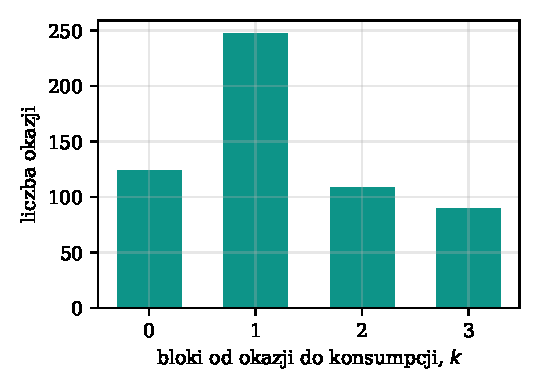
\includegraphics[width=.5\linewidth]{Images/k-hist.pdf}
\caption{Liczba bloków od wykrycia okazji do transakcji konsumującej (trasa \texttt{two\_pool};
  $n=570$ okazji zamkniętych przez 345 transakcji)}
\label{fig:khist}
\end{figure}

\subsection{Protokół ewaluacji}

Wszystkie metryki porównawcze liczone są na populacji zweryfikowanych okazji o~znanej etykiecie:
\texttt{opportunity\_verifications} złączone z~\texttt{opportunities}, z~wykluczeniem trasy
\texttt{multi} (ADR~0008). Osobna populacja wszystkich stanów bloków (tło jako klasa 0) jest
zapisywana wyłącznie diagnostycznie; odróżnienie okazji od tła jest na niej trywialne (AUC
$\approx 0{,}99$) i~nie służy do porównań.

Modele uczone na danych ocenia się w~podziale międzyoknowym: konfiguracja \emph{W2} trenuje na
oknie 2021-05 i~testuje na oknach 2021-11, 2022-05 i~2022-11; konfiguracja \emph{W2+W4}
(międzyreżimowa) trenuje na oknach 2021-05 i~2022-05, a~testuje na 2021-11 i~2022-11. Wewnątrz
treningu ANFIS 20\,\% grup służy do wczesnego zatrzymania. Grupą jest zbiór okazji dzielących
tę samą transakcję konsumującą, a~dla okazji bez transakcji klaster sąsiednich okazji tej samej
pary w~oknie (przerwa $\le 3$ bloki); tło to singletony (ADR~0007). Podział grupowy jest
konieczny, bo 198 zweryfikowanych konsumpcji atomowych w~oknie 2021-05 pochodzi tylko ze 129
transakcji.

Metryki podstawowe to AUC (statystyka Manna--Whitneya z~remisami liczonymi po 0,5) oraz PR-AUC
(średnia precyzja z~interpolacją krokową), obie niezależne od progu. Przy stałym progu
$\mathrm{score}\ge 50$ raportowane są precyzja, czułość i~$F_1$. Baseline~v2 ma próg dobrany na
etykietach okna kalibracji, a~pozostałe modele próg stały, dlatego dla każdego modelu podaje się
też próg F1-optymalny na jego oknach treningowych (ADR~0006). Przedział ufności 95\,\% dla AUC
pochodzi z~bootstrapu stratyfikowanego po klasie (1000 prób, ziarno 42, percentyle 2,5 i~97,5).
Stabilność ANFIS względem inicjalizacji i~tasowania oceniono na pięciu ziarnach (42--46) dla
każdej konfiguracji. Wszystkie liczby w~tym rozdziale generuje polecenie
\texttt{npm run export-results}, korzystające z~tych samych funkcji, które obsługują API.

\subsection{Poprawność implementacji}

\paragraph{Testy automatyczne.} Repozytorium zawiera 140 plików testowych z~953 przypadkami
(Vitest) w~czterech warstwach: jednostkowe (czyste funkcje), integracyjne z~bazą testową
(osobna baza z~sufiksem \texttt{\_test}, chroniona przed pomyleniem z~bazą roboczą), testy na
żywym węźle RPC (włączane zmienną środowiskową) oraz regresje względem danych referencyjnych.
Pokrycie linii wynosi 99,3\,\% dla pakietu \texttt{core} i~99,7\,\% dla \texttt{analysis} przy
progu 80\,\% wymuszanym w~konfiguracji; pozostałe pakiety mają pokrycie 94,7--100\,\%. Testy
arytmetyki AMM porównują \texttt{getAmountOut} z~kwotami rzeczywistych swapów z~łańcucha, testy
systemu Mamdaniego odtwarzają sześć scenariuszy i~rozkład etykiet implementacji referencyjnej,
a~testy
weryfikacji używają zapisanych paragonów transakcji, więc nie zależą od dostępności RPC. Potok
CI (GitHub Actions) uruchamia sprawdzenie typów, lint, migracje na usłudze PostgreSQL~16, testy
z~pokryciem i~budowę interfejsu przy każdym wypchnięciu na gałąź główną.

\paragraph{Niezmienniki danych.} Dwanaście ograniczeń \texttt{CHECK} dodano do schematu po
zebraniu danych; zapytania kontrolne przed ich włączeniem nie wykazały żadnego naruszenia na
1,4~mln stanów, 4\,829 okazjach i~23,2~mln ocen modeli.

\paragraph{Kontrola ręczna weryfikacji.} Heurystyki klasyfikacji (kandydat, beneficjent,
trasa) sprawdzono niezależnie od kodu, porównując wiersze
\texttt{opportunity\_verifications} z~odczytem tych samych transakcji w~serwisie Etherscan.
Próba objęła 10 pierwszych chronologicznie konsumpcji atomowych pary WETH/USDC w~oknie 2021-05
oraz 3 kontrole statusów \texttt{decayed}/\texttt{persisted}. Wyniki: 10/10 zgodnych co do
\texttt{gas\_used} (co do jednostki) i~kierunków swapów, 9/10 zgodnych co do znaku i~rzędu
wielkości zysku (2/10 z~dokładnością poniżej 1~USD), 1/10 poprawnie sklasyfikowana jako trasa
\texttt{multi} (agregator między pulami), 3/3 kontrole negatywne bez fałszywych negatywów.
Trzy transakcje z~zawijaniem i~odwijaniem WETH potwierdziły, że po korekcie ETH~$\equiv$~WETH
zysk zrealizowany zmienia się z~artefaktu rzędu 1,6~mln USD na 35,8~tys.~USD (szczegóły
w~\texttt{docs/verification-method.md}). Kontrolę można powtórzyć testem
\texttt{known-tx.test.ts} na żywym RPC.

\paragraph{Odtwarzalność.} Skrypt \texttt{scripts/reproduce.sh} odtwarza całość od pustej bazy:
64 zadania danych (mediana czasu pobrania puli w~oknie 334~s, analizy pary 10,5~s, weryfikacji
0,7~s), kalibrację baseline~v2 (28~s) i~10 treningów ANFIS (mediana 37~s). Każdy zapis modelu
niesie proweniencję: skrót commitu, wersje bibliotek, zakresy bloków i~liczności tabel
(\texttt{results/provenance.json}).

\subsection{Studium przypadku: droga jednej okazji}

Pozostałe podrozdziały podają metryki zagregowane po całej populacji. Poniżej prześledzono jedną okazję od stanu pul w~bloku
aż po etykietę weryfikacji, co pokazuje, jaką informację system daje o~pojedynczej
rozbieżności. Przypadek dobrano jako \emph{wzorcowy, a~nie typowy}:
rozbieżność jest duża, a~kolejne etapy przetwarzania dają zgodny rachunek, co pozwala zestawić
je obok siebie. Zastrzeżenia o~reprezentatywności zebrano na końcu podrozdziału.


\paragraph{Powstanie rozbieżności.} Okazja dotyczy pary WETH/USDC w~oknie 2021-05 i~obejmuje
cztery kolejne bloki (tab.~\ref{tab:case-blocks}). W~bloku 12\,430\,486 do puli Uniswapa trafiło
391,43~WETH w~zamian za 1\,466\,334,87~USDC; cena w~tej puli spadła zgodnie z~niezmiennikiem
$x\cdot y=k$, a~pula Sushiswapa pozostała bez zmian, bo nie zaszła w~niej wówczas żadna wymiana.
Rozbieżność utrzymała się przez jeden blok i~zamknęła w~bloku 12\,430\,488.

\begin{table}[H]\centering\small
\caption{Stan pary WETH/USDC w~czterech kolejnych blokach okna 2021-05 (ceny w~USDC za 1~WETH)}
\label{tab:case-blocks}
\begin{tabular}{rrrrl}
\toprule
Blok & Uniswap & Sushiswap & $S$ [\%] & Zdarzenie \\
\midrule
12\,430\,485 & 3\,791,00 & 3\,801,05 & 0,265 & stan poniżej progu \\
12\,430\,486 & 3\,723,96 & 3\,801,05 & 2,070 & sprzedaż 391,43 WETH w~Uniswapie \\
12\,430\,487 & 3\,724,57 & 3\,801,00 & 2,052 & \textbf{okazja omawiana poniżej} \\
12\,430\,488 & 3\,774,14 & 3\,777,82 & 0,097 & transakcja arbitrażowa domyka lukę \\
\bottomrule
\end{tabular}
\end{table}

\paragraph{Cechy i~wykrycie.} W~bloku 12\,430\,487 rozbieżność $S=2{,}052\,\%$ przekracza próg
0,65\,\%, więc blok trafia do tabeli \texttt{opportunities}. Pozostałe cechy wynoszą
$G=0{,}139\,\%$, $L=100{,}0$~mln~USD (górna granica dziedziny) i~$M=65{,}1$. Bazowy token jest
tańszy w~Uniswapie, więc kierunek to \texttt{a->b}. Optymalna wielkość transakcji policzona
wzorem z~fragmentu~\ref{lst:opttrade} wynosi 664\,266,81~USDC i~daje zysk brutto 4\,767,91~USD;
po odjęciu szacowanego kosztu gazu 69,65~USD (220\,000 jednostek przy medianie 85~gwei w~tym
bloku) zysk netto wynosi 4\,698,26~USD.

\paragraph{Oceny modeli.} Tę samą okazję cztery modele oceniają różnie
(tab.~\ref{tab:case-scores}). System Mamdaniego uruchamia dokładnie dwie reguły: R11 z~siłą
0,245 (konkluzja ,,wykonalna'') i~R13 z~siłą 0,255 (konkluzja ,,ryzykowna''), a~centroid
agregatu wypada między nimi. Warto odróżnić ocenę od etykiety słownej: próg klasyfikacji
binarnej wynosi 50, więc ocena 52,25 jest predykcją pozytywną, mimo że etykieta wyznaczona
z~funkcji przynależności $W$ brzmi ,,ryzykowna''.

\begin{table}[H]\centering\small
\caption{Oceny okazji z~bloku 12\,430\,487 wystawione przez cztery modele}
\label{tab:case-scores}
\begin{tabular}{llr l}
\toprule
Model & Ocena & & Etykieta \\
\midrule
baseline v1      & 70,73  & & wykonalna \\
Mamdani          & 52,25  & & ryzykowna \\
baseline v2      & 100,00 & & atrakcyjna \\
ANFIS W2+W4      & 88,50  & & atrakcyjna \\
\bottomrule
\end{tabular}
\end{table}

\paragraph{Weryfikacja retrospektywna.} W~bloku bezpośrednio następującym ($k=1$) system
odnajduje transakcję \texttt{0xe2991cbb\ldots eafc46be} o~trasie dwupulowej, która zamyka
rozbieżność. Zysk zrealizowany brutto wynosi 4\,776,76~USD, zużycie gazu 97\,344 jednostki
o~koszcie 553,19~USD, a~zysk netto 4\,223,57~USD, więc etykieta
\texttt{profitable\_consumed} przyjmuje wartość prawda. Komplet tych informacji --- cechy,
aktywacje reguł, oceny modeli i~wynik weryfikacji wraz z~odnośnikiem do eksploratora łańcucha
--- interfejs pokazuje w~panelu szczegółów okazji (rys.~\ref{fig:ui-okazja}).

\begin{figure}[H]\centering
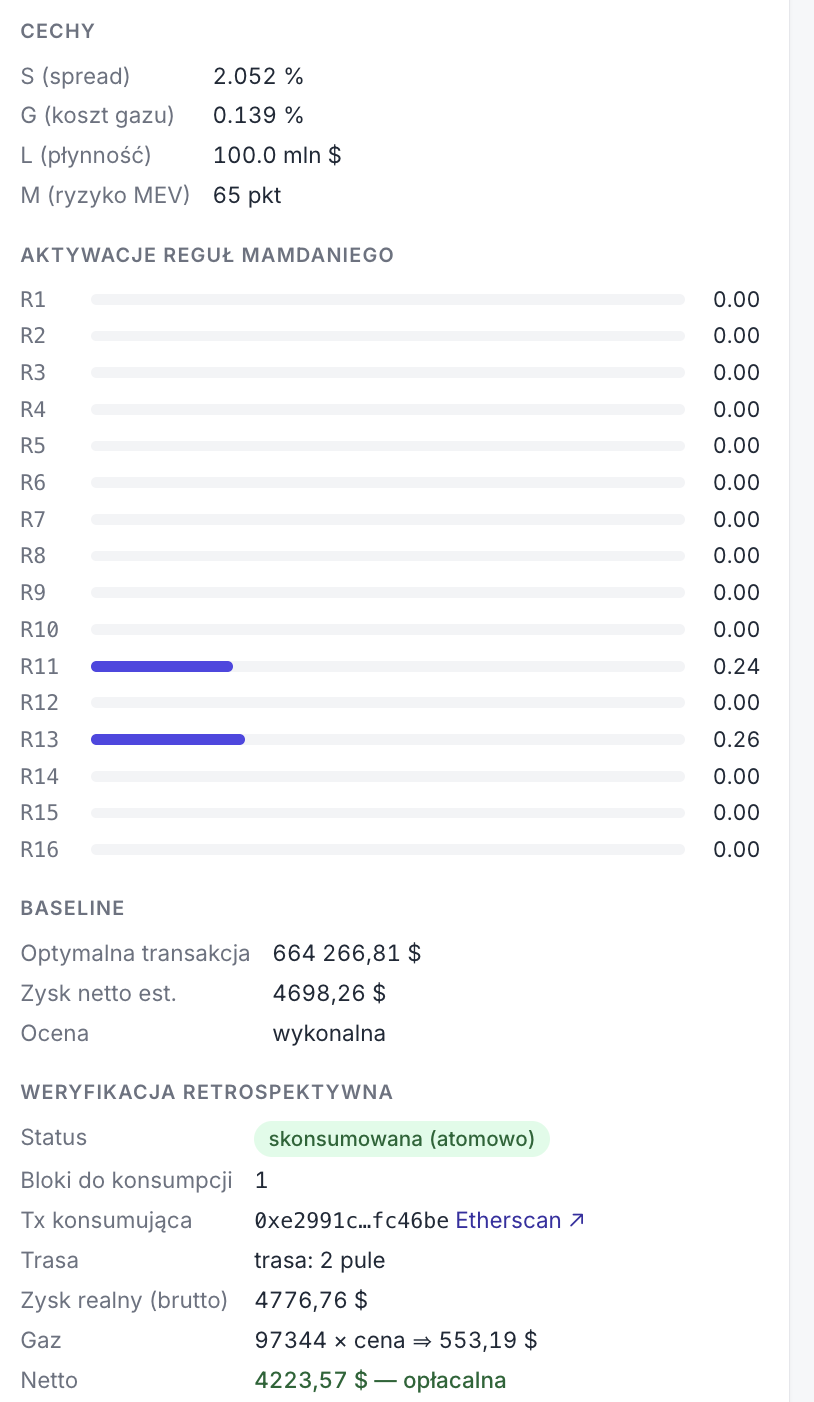
\includegraphics[width=.46\linewidth]{Images/ui-okazja-szczegoly.png}
\caption{Panel szczegółów okazji: cechy, aktywacje 16 reguł systemu Mamdaniego, wynik
heurystyki oraz weryfikacja retrospektywna (zrzut ekranu)}\label{fig:ui-okazja}
\end{figure}

\paragraph{Wnioski z~przypadku.} Szacunek zysku brutto (4\,767,91~USD) różni się od wartości
zrealizowanej (4\,776,76~USD) o~0,19\,\%, co potwierdza poprawność arytmetyki puli. Cała
istotna rozbieżność leży natomiast po stronie kosztu: szacunek zakłada medianę ceny gazu
w~bloku i~daje 69,65~USD, podczas gdy zwycięzca zapłacił 553,19~USD, czyli blisko ośmiokrotnie
więcej, ponieważ o~kolejność w~bloku konkuruje się właśnie ceną gazu. Dokładny jest zatem model
wyceny, a~nie model kosztu --- obserwacja ta wraca w~podrozdziale~4.8.

Przypadek jest wzorcowy i~nie należy go uogólniać: rozbieżność 2\,\% mieści się w~górnym
ogonie rozkładu, a~oceny wszystkich czterech modeli są tu zgodne co do kierunku. W~populacji
takiej zgodności nie ma --- porównanie modeli w~kolejnym podrozdziale pokazuje, że przewaga
jednego nad drugim jest kwestią kilku punktów AUC, a~nie pojedynczych trafień.

\subsection{Porównanie modeli}

Tabela~\ref{tab:models} zestawia pięć modeli: baseline~v1, system Mamdaniego, baseline~v2
(kalibrowany na oknie 2021-05) oraz ANFIS w~dwóch konfiguracjach (ziarno 42). Wiersze oznaczone
,,(tr)'' dotyczą okien użytych do treningu lub kalibracji danego modelu i~nie są miarą
generalizacji. Krzywe ROC dla wszystkich okien łącznie pokazuje rys.~\ref{fig:rocall},
a~w~podziale na okna rys.~\ref{fig:rocwin}. Pełna tabela dla wszystkich 19 modeli, w~tym
historycznych, znajduje się w~pliku \texttt{results/evaluation.md}.

\begin{table}[H]\centering\scriptsize\setlength{\tabcolsep}{3.5pt}
\caption{Metryki modeli na populacji zweryfikowanych okazji ($n$ --- liczność, $n_+$ --- pozytywy;
  próg 50; ,,(tr)'' --- okno treningowe/kalibracyjne modelu)}\label{tab:models}
\begin{tabular}{llrrrrrrl}
\toprule
Okno & Model & $n$ & $n_+$ & Prec. & Czułość & $F_1$ & PR-AUC & AUC [95\,\% CI] \\
\midrule
2021-05 krach & baseline v1  & 2118 & 477 & 0{,}536 & 0{,}109 & 0{,}181 & 0{,}331 & 0{,}627 [0{,}60--0{,}65] \\
 & Mamdani      & 2118 & 477 & 0{,}222 & 0{,}017 & 0{,}031 & 0{,}197 & 0{,}392 [0{,}36--0{,}42] \\
 & baseline v2 (tr) & 2118 & 477 & 0{,}350 & 0{,}706 & 0{,}468 & 0{,}397 & 0{,}700 [0{,}67--0{,}72] \\
 & ANFIS W2 (tr) & 2118 & 477 & 0{,}246 & 0{,}975 & 0{,}393 & 0{,}426 & 0{,}712 [0{,}69--0{,}74] \\
 & ANFIS W2+W4 (tr) & 2118 & 477 & 0{,}228 & 0{,}994 & 0{,}370 & 0{,}415 & 0{,}707 [0{,}68--0{,}73] \\
\midrule
2021-11 ATH & baseline v1  & 886 & 20 & 0{,}000 & 0{,}000 & 0{,}000 & 0{,}038 & 0{,}599 [0{,}51--0{,}70] \\
 & Mamdani      & 886 & 20 & 0{,}000 & 0{,}000 & 0{,}000 & 0{,}017 & 0{,}359 [0{,}25--0{,}46] \\
 & baseline v2  & 886 & 20 & 0{,}153 & 0{,}650 & 0{,}248 & 0{,}107 & 0{,}825 [0{,}74--0{,}90] \\
 & ANFIS W2     & 886 & 20 & 0{,}029 & 0{,}850 & 0{,}056 & 0{,}073 & 0{,}737 [0{,}62--0{,}85] \\
 & ANFIS W2+W4  & 886 & 20 & 0{,}023 & 1{,}000 & 0{,}045 & 0{,}100 & 0{,}762 [0{,}64--0{,}87] \\
\midrule
2022-05 Luna & baseline v1  & 1279 & 40 & 0{,}175 & 0{,}175 & 0{,}175 & 0{,}107 & 0{,}713 [0{,}63--0{,}79] \\
 & Mamdani      & 1279 & 40 & 0{,}000 & 0{,}000 & 0{,}000 & 0{,}039 & 0{,}593 [0{,}52--0{,}67] \\
 & baseline v2  & 1279 & 40 & 0{,}098 & 0{,}575 & 0{,}168 & 0{,}138 & 0{,}800 [0{,}72--0{,}87] \\
 & ANFIS W2     & 1279 & 40 & 0{,}045 & 0{,}250 & 0{,}077 & 0{,}055 & 0{,}702 [0{,}63--0{,}76] \\
 & ANFIS W2+W4 (tr) & 1279 & 40 & 0{,}081 & 0{,}600 & 0{,}142 & 0{,}137 & 0{,}778 [0{,}71--0{,}84] \\
\midrule
2022-11 FTX & baseline v1  & 402 & 7 & 0{,}125 & 0{,}286 & 0{,}174 & 0{,}097 & 0{,}788 [0{,}61--0{,}95] \\
 & Mamdani      & 402 & 7 & 0{,}000 & 0{,}000 & 0{,}000 & 0{,}037 & 0{,}731 [0{,}61--0{,}84] \\
 & baseline v2  & 402 & 7 & 0{,}071 & 0{,}286 & 0{,}114 & 0{,}128 & 0{,}839 [0{,}70--0{,}95] \\
 & ANFIS W2     & 402 & 7 & 0{,}000 & 0{,}000 & 0{,}000 & 0{,}032 & 0{,}677 [0{,}50--0{,}82] \\
 & ANFIS W2+W4  & 402 & 7 & 0{,}087 & 0{,}286 & 0{,}133 & 0{,}126 & 0{,}879 [0{,}79--0{,}95] \\
\midrule
wszystkie okna & baseline v1  & 4685 & 544 & 0{,}370 & 0{,}112 & 0{,}172 & 0{,}210 & 0{,}654 [0{,}63--0{,}68] \\
 & Mamdani      & 4685 & 544 & 0{,}101 & 0{,}015 & 0{,}026 & 0{,}097 & 0{,}354 [0{,}33--0{,}38] \\
 & baseline v2  & 4685 & 544 & 0{,}286 & 0{,}689 & 0{,}405 & 0{,}326 & 0{,}796 [0{,}78--0{,}81] \\
 & ANFIS W2     & 4685 & 544 & 0{,}180 & 0{,}904 & 0{,}300 & 0{,}269 & 0{,}787 [0{,}77--0{,}81] \\
 & ANFIS W2+W4  & 4685 & 544 & 0{,}159 & 0{,}956 & 0{,}273 & 0{,}369 & 0{,}818 [0{,}80--0{,}83] \\
\bottomrule
\end{tabular}
\end{table}

Progi F1-optymalne wyznaczone na oknach treningowych wynoszą 50,0 dla baseline~v2 (z~konstrukcji),
80,4 dla ANFIS~W2 i~81,5 dla ANFIS~W2+W4; oba modele ANFIS przy progu 50 klasyfikują jako
pozytywne 58--70\,\% populacji, co widać w~wysokiej czułości i~niskiej precyzji w~tabeli.
Kalibracja baseline~v2 wybrała z~siatki 30 kombinacji punkt $\mathrm{gasUnits}=150\,000$,
$\kappa=0$, $w=0$ (próg $v=0{,}728$, skala 70,6), czyli ranking okazji według samego zysku brutto;
sąsiednie punkty siatki z~$\kappa=0{,}25$ miały AUC niższe o~0,01--0,04 na oknie kalibracji.

Wiersz ,,wszystkie okna'' łączy okna testowe z~treningowymi: dla baseline~v2 i~ANFIS~W2 okno
kalibracji lub treningu 2021-05 stanowi 45,2\,\% populacji (2\,118 z~4\,685), dla ANFIS~W2+W4 okna
2021-05 i~2022-05 stanowią 72,5\,\% (3\,397 z~4\,685); baseline~v1 i~Mamdani nie mają okien
treningowych. Miarą generalizacji są więc wyłącznie wiersze okien testowych.

\begin{figure}[H]\centering
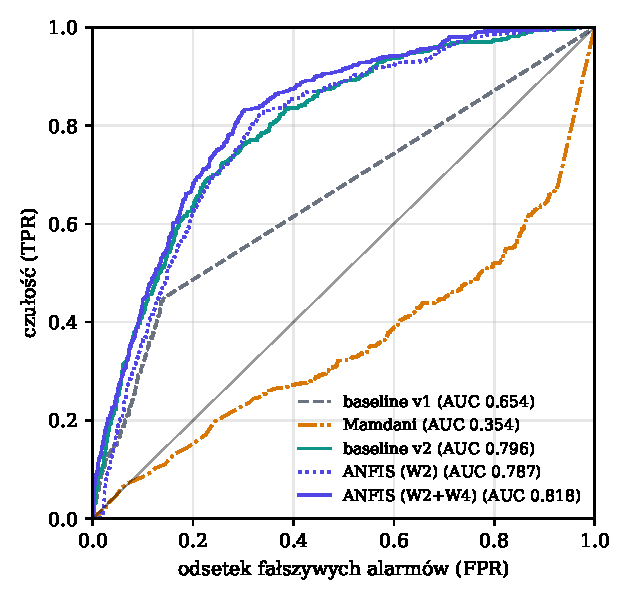
\includegraphics[width=.62\linewidth]{Images/roc-all.pdf}
\caption{Krzywe ROC pięciu modeli na wszystkich oknach łącznie ($n=4\,685$, $n_+=544$)}
\label{fig:rocall}
\end{figure}

\begin{figure}[H]\centering
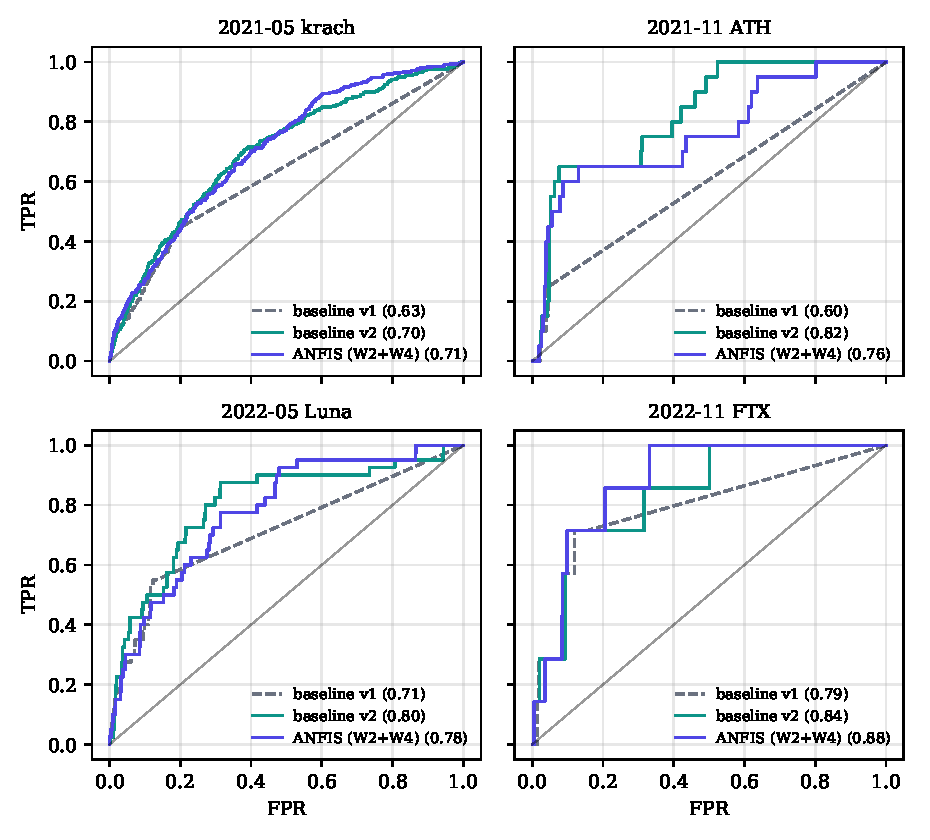
\includegraphics[width=.9\linewidth]{Images/roc-windows.pdf}
\caption{Krzywe ROC baseline~v1, baseline~v2 i~ANFIS W2+W4 w~podziale na okna (w~nawiasach AUC)}
\label{fig:rocwin}
\end{figure}

\paragraph{Wrażliwość na definicję populacji.} Populacja ewaluacji (ADR~0008) zawiera konsumpcje
w~bloku wykrycia ($k=0$), w~których stan puli na koniec bloku jest już stanem po konsumpcji, oraz
konsumpcje, przed którymi w~bloku $B+k$ inne transakcje zmieniły stan pul. Tabela~\ref{tab:sensitivity}
powtarza metryki dla trzech wariantów populacji: \emph{pełna} (jak w~tab.~\ref{tab:models}),
\emph{bez $k=0$} (bez konsumpcji atomowych w~bloku wykrycia) oraz \emph{bot pierwszy} (z~konsumpcji
\texttt{two\_pool} zostają tylko te z~$k\ge1$, w~których transakcja konsumująca była pierwszym swapem
bloku $B+k$ w~pulach pary; pozostałe konsumpcje \texttt{two\_pool} mają etykietę nieokreśloną i~są
wykluczone, negatywy pozostają bez zmian). W~wariantach \emph{pełna} i~\emph{bez $k=0$} kolejność
modeli według AUC jest identyczna. W~wariancie \emph{bot pierwszy} AUC każdego modelu rośnie,
najbardziej baseline~v2 (z~0,796 do 0,867), który wyprzedza wówczas ANFIS~W2+W4 (0,829); system
Mamdaniego pozostaje poniżej 0,5 w~każdym wariancie.

\begin{table}[H]\centering\footnotesize\setlength{\tabcolsep}{4pt}
\caption{Metryki modeli na wszystkich oknach łącznie dla trzech wariantów populacji ewaluacji
  (próg 50; AUC z~95\,\% CI z~bootstrapu)}\label{tab:sensitivity}
\begin{tabular}{llrrrl}
\toprule
Model & Wariant & $n$ & $n_+$ & PR-AUC & AUC [95\,\% CI] \\
\midrule
baseline v1   & pełna        & 4\,685 & 544 & 0{,}210 & 0{,}654 [0{,}63--0{,}68] \\
              & bez $k=0$    & 4\,561 & 423 & 0{,}177 & 0{,}664 [0{,}64--0{,}69] \\
              & bot pierwszy & 4\,290 & 156 & 0{,}107 & 0{,}756 [0{,}72--0{,}79] \\
\midrule
Mamdani       & pełna        & 4\,685 & 544 & 0{,}097 & 0{,}354 [0{,}33--0{,}38] \\
              & bez $k=0$    & 4\,561 & 423 & 0{,}079 & 0{,}362 [0{,}33--0{,}39] \\
              & bot pierwszy & 4\,290 & 156 & 0{,}035 & 0{,}410 [0{,}35--0{,}47] \\
\midrule
baseline v2   & pełna        & 4\,685 & 544 & 0{,}326 & 0{,}796 [0{,}78--0{,}81] \\
              & bez $k=0$    & 4\,561 & 423 & 0{,}283 & 0{,}808 [0{,}79--0{,}83] \\
              & bot pierwszy & 4\,290 & 156 & 0{,}171 & 0{,}867 [0{,}84--0{,}89] \\
\midrule
ANFIS W2      & pełna        & 4\,685 & 544 & 0{,}269 & 0{,}787 [0{,}77--0{,}81] \\
              & bez $k=0$    & 4\,561 & 423 & 0{,}221 & 0{,}788 [0{,}77--0{,}81] \\
              & bot pierwszy & 4\,290 & 156 & 0{,}107 & 0{,}795 [0{,}76--0{,}83] \\
\midrule
ANFIS W2+W4   & pełna        & 4\,685 & 544 & 0{,}369 & 0{,}818 [0{,}80--0{,}83] \\
              & bez $k=0$    & 4\,561 & 423 & 0{,}310 & 0{,}817 [0{,}80--0{,}84] \\
              & bot pierwszy & 4\,290 & 156 & 0{,}163 & 0{,}829 [0{,}79--0{,}86] \\
\bottomrule
\end{tabular}
\end{table}

\subsection{Stabilność modelu ANFIS}

Dla obu konfiguracji ANFIS powtórzono trening z~pięcioma ziarnami generatora (42--46), które
sterują podziałem walidacyjnym i~tasowaniem minipaczek; dane i~hiperparametry były identyczne.
Wyniki (rys.~\ref{fig:seeds}, \texttt{results/evaluation-seeds.csv}): konfiguracja W2 osiąga na
wszystkich oknach AUC $0{,}719 \pm 0{,}081$ (rozstęp od 0,584 do 0,787), a~konfiguracja W2+W4
$0{,}822 \pm 0{,}005$ (od 0,818 do 0,830). Odchylenie standardowe PR-AUC wynosi odpowiednio 0,070
i~0,004. Na oknie treningowym 2021-05 obie konfiguracje są stabilne (sd AUC 0,004 i~0,003);
rozrzut konfiguracji W2 pochodzi z~okien testowych 2022-05 (sd 0,062) i~2022-11 (sd 0,107).
Obie konfiguracje nie są jednak porównywane na równych warunkach. W2+W4 ma okno 2022-05
w~treningu, więc jej wynik na wszystkich oknach łączy dwa okna treningowe z~dwoma testowymi,
podczas gdy W2 ma jedno okno treningowe i~trzy testowe. Mniejszy rozrzut W2+W4 po części
bierze się właśnie stąd; miarodajne dla generalizacji są tylko okna 2021-11 i~2022-11.

\begin{figure}[H]\centering
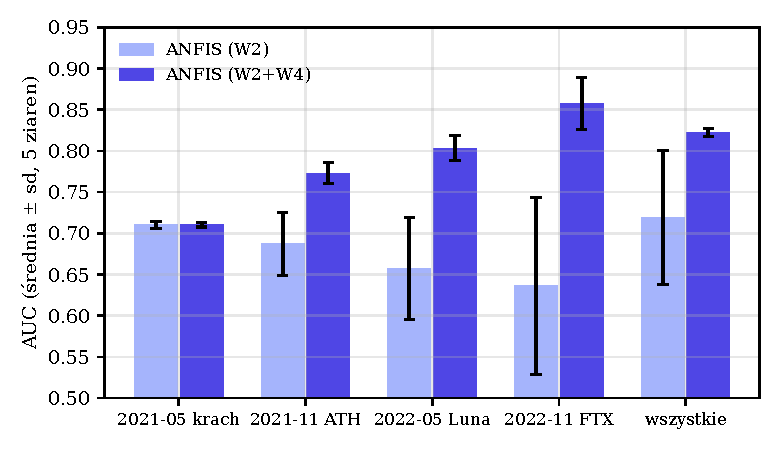
\includegraphics[width=.75\linewidth]{Images/seeds.pdf}
\caption{AUC ANFIS według okien: średnia i~odchylenie standardowe z~pięciu ziaren}
\label{fig:seeds}
\end{figure}

\subsection{Wstępna ocena ekonomiczna}

Tabela~\ref{tab:econ} charakteryzuje okazje od strony ekonomicznej: szacowany zysk brutto
z~optymalnej transakcji dwupulowej, wielkość tej transakcji, koszt gazu według założeń
baseline~v1 (220\,000 jednostek przy medianowej cenie gazu bloku) oraz udział okazji, dla których
szacowany zysk netto jest dodatni. Ostatnia kolumna podaje ten udział przy koszcie gazu
zmniejszonym o~połowę i~podwojonym, jako analizę wrażliwości na cenę gazu.

\begin{table}[H]\centering\footnotesize\setlength{\tabcolsep}{3pt}
\caption{Ekonomia okazji według okien (mediany; cztery pary łącznie). $\Pi$ --- szacowany zysk
  brutto, $\Delta y^{*}$ --- optymalna transakcja, $C_g$ --- koszt gazu wg baseline~v1;
  udział okazji z~$\Pi - C_g > 0$ przy $C_g$ oraz przy $0{,}5\,C_g$ / $2\,C_g$}\label{tab:econ}
\begin{tabular}{lrrrrrrrrr}
\toprule
Okno & $n$ & $S$ [\%] & gaz [gwei] & $\Pi$ [USD] & $\Pi_{p90}$ [USD] & $\Delta y^{*}$ [USD] & $C_g$ [USD] & $\Pi>C_g$ & $0{,}5\,C_g$ / $2\,C_g$ \\
\midrule
2021-05 krach & 2\,236 & 0{,}817 & 387 & 57{,}5 & 999 & 54\,592 & 200 & 27{,}0\,\% & 40{,}5 / 17{,}5\,\% \\
2021-11 ATH   & 891   & 0{,}698 & 136 & 11{,}2 & 67  & 23\,459 & 134 & 5{,}3\,\%  & 9{,}8 / 2{,}8\,\% \\
2022-05 Luna  & 1\,296 & 0{,}795 & 279 & 8{,}9  & 145 & 9\,231  & 118 & 14{,}7\,\% & 19{,}6 / 10{,}3\,\% \\
2022-11 FTX   & 406   & 0{,}758 & 70  & 2{,}5  & 44  & 3\,092  & 20  & 17{,}0\,\% & 24{,}6 / 11{,}3\,\% \\
\bottomrule
\end{tabular}
\end{table}

Dla konsumpcji atomowych o~trasie \texttt{two\_pool} można zestawić szacunek z~faktem
(tab.~\ref{tab:realized}). Mediana zysku zrealizowanego przez beneficjenta przewyższa medianę
szacowanego zysku brutto z~optymalnej transakcji dwupulowej we wszystkich oknach. Sama mediana
ilorazu tych wielkości (4,7 w~oknie 2021-05) niewiele jednak mówi, bo miesza konsumpcje o~różnym
opóźnieniu. Po rozbiciu według $k$ obraz jest inny. Dla $k=1$ (208 z~500 konsumpcji w~tym oknie)
mediana ilorazu wynosi 1,00, a~w~46\,\% przypadków fakt różni się od szacunku o~mniej niż
5\,\%: bot wykonał niemal dokładnie tę transakcję, którą system wyliczył ze stanu bloku. Dla
$k=0$ mediana sięga 19, bo stan na koniec bloku to już resztka po konsumpcji i~szacunek jest
z~definicji zaniżony. Dla $k=2$ i~$k=3$ mediana rośnie do 5 i~21: rozbieżność zdążyła się
powiększyć, zanim ktoś ją zamknął. Iloraz 4,7 jest więc wypadkową jednego przypadku, w~którym
szacunek trafia, i~trzech, w~których porównywany jest niewłaściwy stan puli.
O~wartości ilorazu rozstrzyga przy tym nie samo opóźnienie, lecz miejsce transakcji w~bloku.
Wśród konsumpcji par kwotowanych w~stablecoinie z~$k\ge1$ (410 we wszystkich oknach) transakcja
bota była pierwszym swapem bloku $B+k$ w~pulach pary w~163 przypadkach: mediana ilorazu wynosi tam
1,00 przy rozstępie międzykwartylowym 1,00--1,01, a~wielkość transakcji bota odpowiada optymalnej
transakcji wyliczonej przez system (mediana ilorazu 0,99). Dla pozostałych 247 konsumpcji,
w~których wcześniejsze swapy innych transakcji zmieniły stan pul, mediana ilorazu wynosi 9,64
(kwartyle 2,40 i~37,14), a~transakcja bota jest trzykrotnie większa od optymalnej dla stanu
z~bloku wykrycia.
Rzeczywiste zużycie gazu (mediana
142--155~tys. jednostek) jest niższe od założonych 220\,000, a~w~oknie 2021-05 131 z~618
konsumpcji atomowych ma zerową cenę gazu w~transakcji. Łączny zysk netto beneficjentów trzeba
sumować po transakcjach, nie po okazjach, bo jedna transakcja zamyka często rozbieżność widoczną
w~kilku kolejnych blokach. Za 570 konsumpcji \texttt{two\_pool} odpowiada 345 transakcji o~łącznym
zysku netto 1,15~mln USD, z~czego 1,13~mln USD przypada na okno 2021-05. Sumowanie po okazjach
dałoby 1,87~mln USD, czyli zawyżyłoby wynik o~ponad połowę.
Zestawienie szacunku netto baseline~v1 z~etykietą: spośród 544 okazji skonsumowanych z~zyskiem
299 miało szacowany zysk netto ujemny, a~spośród 840 okazji o~dodatnim szacunku netto 595 nie
zostało skonsumowanych z~zyskiem.

\begin{table}[H]\centering\scriptsize\setlength{\tabcolsep}{3.5pt}
\caption{Konsumpcje atomowe o~trasie \texttt{two\_pool}: szacunek a~fakt (mediany); $k=0$ ---
  udział konsumpcji w~bloku okazji}\label{tab:realized}
\begin{tabular}{lrrrrrrrr}
\toprule
Okno & $n$ & zysk zreal. [USD] & $\Pi$ szac. [USD] & iloraz & gaz zreal. [USD] & $C_g$ szac. [USD] & gaz [jedn.] & $k=0$ \\
\midrule
2021-05 krach & 500 & 1\,020 & 171 & 4{,}70 & 225 & 295 & 149\,531 & 23\,\% \\
2021-11 ATH   & 20  & 225    & 120 & 1{,}01 & 131 & 142 & 155\,402 & 0\,\% \\
2022-05 Luna  & 43  & 700    & 76  & 2{,}56 & 129 & 98  & 154\,361 & 21\,\% \\
2022-11 FTX   & 7   & 176    & 43  & 1{,}91 & 11  & 17  & 142\,587 & 14\,\% \\
\bottomrule
\end{tabular}
\end{table}

\subsection{Dyskusja wyników i~ograniczenia}

Wyniki układają się w~spójny obraz po ustaleniu, co mierzy etykieta. To tutaj zaczyna się
dyskusja, a~kończy ją lista ograniczeń systemu.

\paragraph{Co mierzy etykieta?} Etykieta pozytywna oznacza, że okazja została skonsumowana
transakcją atomową o~trasie dwupulowej i~beneficjent na niej zarobił. 544 z~570 skonsumowanych
okazji były zyskowne, więc jest ona w~praktyce równoważna stwierdzeniu ,,ktoś to wziął''. Zatem
można stwierdzić, że modele oceniane na tej populacji przewidują zachowanie konkurencji, a~nie
wykonalność okazji arbitrażowej dla zewnętrznego obserwatora. Ta różnica tłumaczy trzy
obserwacje: odwrócenie systemu Mamdaniego, kalibrację baseline~v2 i~granicę, na której zatrzymał
się ANFIS.

\paragraph{Modele.} System Mamdaniego działa odwrotnie do etykiety: jego reguły odpowiadają na
pytanie ,,czy ja zdążę i~na tym zarobię''. Karzą wysoki koszt gazu i~dużą aktywność w~bloku,
tymczasem okazje skonsumowane w~oknie 2021-05 miały wyższą medianę $G$ i~$M$ niż pozostałe, bo
wysoki ruch w~bloku świadczy o~wysokiej obecności botów. Term ,,zaporowy'' dla $G$ spełnia
1,2\,\% bloków w~oknie 2021-05 i~żaden blok w~oknach z~2022~roku. Reguła wetująca dla gazu
praktycznie się nie uruchamia. Dla trzech z~czterech par cecha $L$ wynosi 100 w~każdym bloku
z~okna 2021-05, więc term ,,głęboka'' jest zawsze spełniony i~$L$ nie różnicuje okazji.
Kalibracja baseline~v2 wyzerowała wagę kosztu gazu i~sprowadziła model do rankingu po zysku
brutto. ANFIS uczony na tych samych danych osiągnął AUC 0,818 w~porównaniu do 0,796 dla
baseline~v2, przy nakładających się przedziałach ufności. Przy progu 50 oznacza on jako pozytywne
58--70\,\% okazji. Uczenie z~danych odzyskało ranking po wielkości okazji i~niewiele ponad to.

\paragraph{Szacunek a~fakt.} Mediana ilorazu zysku zrealizowanego do szacowanego, wynosząca 4,7
w~oknie 2021-05, jest wynikiem mieszania konsumpcji o~różnym opóźnieniu i~różnym miejscu
w~bloku. W~podzbiorze opisanym w~podrozdziale~4.7, gdy transakcja bota była pierwszym swapem
bloku, mediana ilorazu wynosi 1,00 przy rozstępie międzykwartylowym 1,00--1,01, a~dla pozostałych
konsumpcji 9,64, ponieważ między wykryciem a~konsumpcją cudze transakcje zmieniły stan pul.
Arytmetyka AMM o~stałym iloczynie odtwarza więc zysk co do wartości, a~rozjazd bierze się z~czasu.
Statystyki ekonomiczne liczone po okazjach zawyżają wynik, bo 570 konsumpcji dwupulowych to 345
transakcji: suma po transakcjach daje 1,15~mln USD zamiast 1,87~mln USD.

\paragraph{Statystyka.} Klasa pozytywna skupia się w~oknie 2021-05 (477 z~544), a~w~oknach 3--5
liczy 20, 40 i~7 przypadków. Stąd przedziały ufności szerokości do ponad 0,3, a~AUC 0,879 przy
siedmiu pozytywach jest liczbą, której nie należy interpretować. Wiersz ,,wszystkie okna'' miesza
rozpoznawanie okna z~rozpoznawaniem okazji, bo udział pozytywów wynosi 22\,\% w~oknie 2021-05
i~1,7--3,1\,\% w~pozostałych; zawiera też dane treningowe (45,2\,\% populacji dla baseline~v2
i~ANFIS~W2, 72,5\,\% dla W2+W4). Porównania modeli są wiarygodne tylko w~podziale na okna
testowe. Wynik ziarna 42 w~tabeli głównej jest dla ANFIS~W2 górnym krańcem rozstępu
(0,787 z~0,584--0,787), a~dla W2+W4 dolnym (0,818 z~0,818--0,830), więc tabela pokazuje
konfigurację W2 od najlepszej strony. Analiza wrażliwości na definicję populacji zachowuje ranking
między wariantami ,,pełna'' i~,,bez $k=0$''; w~wariancie ,,bot pierwszy'' baseline~v2 (0,867)
wyprzedza ANFIS~W2+W4 (0,829), a~system Mamdaniego pozostaje poniżej 0,5 (0,410).

\paragraph{Ograniczenia.} System obejmuje wyłącznie arbitraż dwupulowy między giełdami
Uniswap~V2 i~Sushiswap, więc 144 konsumpcje o~trasie wielopulowej, czyli co piąta konsumpcja
atomowa, mają etykietę nieokreśloną. Okno 2021-05 poprzedza nowy system opłat transakcyjnych
w~sieci Ethereum (EIP-1559), a~trzy pozostałe następują po nim, więc ewaluacja łączy dwa reżimy
opłat, a~cecha $G$ nie jest między nimi w~pełni porównywalna. Heurystyki beneficjenta i~trasy
przenoszą swoje błędy wprost na etykiety, a~kontrola ręczna objęła 13 przypadków. Cecha $M$
narusza zasadę oceny ex~ante: korzysta z~percentyli liczonych po całym oknie, a~w~bloku wykrycia
obejmuje także swapy transakcji konsumującej. System nie symuluje wykonania transakcji, nie widzi
mempoola ani pakietów prywatnych, takich jak Flashbots. Model ANFIS jest uczony metodą Adam na
wszystkich parametrach, a~nie hybrydą z~estymacją najmniejszych kwadratów opisaną
w~rozdziale~2.4, więc wyniki nie przenoszą się wprost na klasyczny ANFIS. Wnioski obowiązują
w~granicach danych: cztery pary, dwie giełdy i~cztery dwutygodniowe okna.

\newpage
\section{Podsumowanie i~wnioski}

\subsection{Realizacja celów pracy}
Cel pracy sformułowany w~rozdziale~1.2 został zrealizowany. Rozbito go na cztery zadania.
\begin{itemize}[nosep]
  \item Zbudowano system gromadzący stany puli płynności na podstawie zdarzeń \texttt{Sync}
        i~\texttt{Swap} pobieranych z~archiwalnego węzła Ethereum. Dla czterech par i~czterech
        okien zebrano 1,42~mln stanów par w~blokach i~wykryto 4\,829 rozbieżności
        przekraczających próg 0,65\,\% (rozdział~4.1).
  \item Opracowano procedurę weryfikacji retrospektywnej, która ustala, czy i~w~którym bloku
        okazja została skonsumowana, kto był jej beneficjentem oraz jaką trasą przebiegła
        (rozdział~3.7). Status konsumpcji atomowej otrzymało 714 okazji, w~tym 570 o~trasie
        dwupulowej. Próba 10 konsumpcji sprawdzonych ręcznie dała zgodność 10/10 co do zużycia
        gazu i~9/10 co do znaku oraz rzędu wielkości zysku (rozdział~4.3).
  \item Zaprojektowano i~zaimplementowano heurystykę progową (baseline~v1) wraz z~jej
        skalibrowaną wersją (baseline~v2), system Mamdaniego oraz sieć ANFIS (rozdział~3.6).
        Modele oceniono na tej samej populacji okazji, w~podziale międzyoknowym i~grupowym,
        z~przedziałami ufności AUC (rozdziały~4.2 i~4.5). Najlepszy wynik generalizacji
        osiągnęły baseline~v2 i~ANFIS.
  \item Zbudowano serwer API z~16 punktami końcowymi oraz interfejs webowy z~pięcioma widokami
        (rozdziały~3.8 i~3.9).
\end{itemize}
Od założeń projektu odstąpiono w~jednym punkcie: zamiast indeksowania zdarzeń usługą The~Graph
zastosowano bezpośrednie zapytania do węzła archiwalnego, co uzasadniono w~rozdziale~1.3.

\subsection{Wnioski}
Na podstawie wyników z~rozdziału~4 sformułowano pięć wniosków.
\begin{itemize}[nosep]
  \item Etykiety uzyskane w~weryfikacji retrospektywnej mierzą zachowanie konkurencji, a~nie
        zyskowną konsumowalność dla zewnętrznego obserwatora. Model uczony na takich etykietach
        przewiduje, czy rozbieżność zostanie skonsumowana, a~nie czy dałoby się ją skonsumować
        samodzielnie.
  \item Ocena wykonalności może być trafniejsza niż samo wykrycie rozbieżności cenowej, ale
        trafność bierze się z~uszeregowania okazji według ich wielkości, a~nie z~wiedzy
        eksperckiej ani ze struktury rozmytej. Reguły przeniesione z~systemu Mamdaniego karzą
        wysoki koszt gazu i~dużą aktywność bloku, a~właśnie takie okazje były konsumowane
        najczęściej; w~oknach z~2021~roku model działa niemal odwrotnie do etykiety
        (AUC 0,392 i~0,359). Kalibracja baseline~v2 wyzerowała wagę kosztu gazu i~sprowadziła
        ocenę do rankingu po zysku brutto, a~ANFIS nie poprawił istotnie wyniku skalibrowanej
        heurystyki.
  \item Koszt gazu nie różnicuje klas, ponieważ arbitrażyści rozliczają go poza polem
        transakcji: w~oknie 2021-05 131 z~618 konsumpcji atomowych ma zerową cenę gazu.
  \item Szacunek zysku z~arytmetyki AMM jest dokładny; źródłem rozbieżności między szacunkiem
        a~faktem jest czas, nie wycena. Dla konsumpcji w~bloku następującym po okazji ($k=1$,
        okno 2021-05) mediana ilorazu zysku zrealizowanego do szacowanego wynosi 1,00.
  \item Sygnał ,,duża rozbieżność cenowa'' oznacza, że różnica zniknie w~ciągu kilku bloków,
        i~jest to użyteczna informacja ochronna. Modele wskazują, które rozbieżności zostaną
        skonsumowane, a~rozkład opóźnień mówi, jak szybko: 81\,\% konsumpcji dwupulowych
        nastąpiło najpóźniej w~drugim bloku po wykryciu okazji. Animator rynku, widząc taki
        sygnał w~trybie na żywo (rys.~\ref{fig:ui-live}), powinien traktować swoją ofertę jako
        narażoną w~perspektywie kilkudziesięciu sekund, a~nie minut.
\end{itemize}

\subsection{Kierunki dalszych prac}
Analiza ograniczeń omówionych w~rozdziale~4.8 wskazuje kierunki, w~których pracę można rozwinąć.
\begin{itemize}[nosep]
  \item Obecna etykieta mówi o~tym, czy rozbieżność została skonsumowana przez konkurencję.
        Dodatkowa etykieta ,,wykonalna dla obserwatora'' obejmowałaby okazje, które przetrwały
        co~najmniej jeden blok od wykrycia i~pozostały zyskowne po odliczeniu kosztu gazu.
        Pozwoliłaby ona sprawdzić, czy reguły eksperckie są trafne przy właściwie postawionym
        pytaniu.
  \item Cecha $M$ korzysta z~percentyli liczonych po całym oknie, więc ocena bloku zależy od
        bloków późniejszych, których w~trybie na żywo jeszcze nie ma. Gdy blok konsumpcji jest
        zarazem blokiem wykrycia, cecha jest wysoka po części dlatego, że swapy transakcji
        konsumującej wchodzą do liczby swapów tego bloku. W~kolejnej wersji percentyle powinny
        być liczone krocząco, a~trening powinien wykluczać konsumpcje w~bloku wykrycia.
  \item Ze zbioru wykluczono 144 konsumpcje o~trasie wielopulowej. Ich rozliczenie wymaga cen
        tokenów spoza analizowanej pary oraz obsługi pul zgodnych z~protokołem Uniswap~V3.
        Włączenie tych tras uzupełniłoby klasę pozytywną i~pozwoliłoby ocenić, jaką część
        arbitrażu przejmują agregatory.
  \item System szacuje zysk na stanie bloku, ale nie sprawdza, czy transakcja wykonałaby się
        poprawnie w~kontekście pozostałych transakcji bloku. Symulacja na lokalnym forku maszyny
        EVM pozwoliłaby uwzględnić kolejność transakcji, poślizg i~odrzucenia, czyli źródła
        różnicy między szacunkiem a~faktem.
\end{itemize}

\newpage
\section{Wykorzystanie narzędzi GenAI}
Narzędzia GenAI zostały wykorzystane wyłącznie w zakresie korekty językowej oraz stylistycznej tekstu niniejszej pracy. Całość treści merytorycznych oraz kody źródłowe stanowią w pełni autorskie opracowanie.

Głównym z~użytych narzędzi był Hermes Agent o~otwartym kodzie źródłowym, w~konfiguracji
z~modelem językowym Qwen3.8-27B uruchamianym lokalnie na komputerze autora (serwer MTPLX
korzystający z~frameworku MLX). W~węższym zakresie posłużono się narzędziem Claude Code firmy
Anthropic, opartym na zdalnie udostępnianych modelach Claude.

Obydwa narzędzia pełniły rolę pomocniczą wobec pracy autora. Projekt systemu (architektura,
model danych, algorytmy, dobór cech i~parametrów modeli oceny) oraz ostateczna postać kodu
w~repozytorium są dziełem autora.

Zakres użycia narzędzi w~opisanej wyżej postaci uzgodniono z~promotorem pracy.

\newpage
\bibliography{references}

\newpage
\appendix
\section*{Załączniki}
\addcontentsline{toc}{section}{Załączniki}
\renewcommand{\thesubsection}{\Alph{subsection}}
\setcounter{subsection}{0}

\subsection{Uruchomienie systemu i~reprodukcja wyników}

Wymagania: Node.js $\geq 20$ (wyniki wygenerowano na v24.13.0), npm $\geq 10$, Docker
(PostgreSQL~16 z~\texttt{docker-compose.yml}) oraz archiwalny węzeł RPC Ethereum obejmujący bloki
z~lat 2021--2022 (zmienna \texttt{RPC\_URL}); publiczne węzły z~\texttt{RPC\_FALLBACK\_URLS}
służą wyłącznie jako zapas po błędach. Uruchomienie środowiska deweloperskiego pokazuje
fragment~\ref{lst:run}, pełną reprodukcję fragment~\ref{lst:repro}.
\begin{lstlisting}[language=bash, caption={Uruchomienie systemu}, label={lst:run}]
cp .env.example .env          # uzupełnić RPC_URL
npm install
npm run db:up && npm run db:migrate && npm run db:seed
npm run dev                    # api (:3001) + worker + web (:5173)
\end{lstlisting}
Pełna reprodukcja od pustej bazy trwa ok. 6--7~h, w~większości na pobieranie danych:
\begin{lstlisting}[language=bash, caption={Reprodukcja wyników}, label={lst:repro}]
npm run reproduce                    # scripts/reproduce.sh: ingest, analiza, weryfikacja,
                                     # kalibracja baseline v2, 10 treningów ANFIS
npm run reproduce -- --skip-ingest   # pomija pobieranie, zakłada gotową bazę
npm run export-results -- --latex    # tabele CSV/Markdown/LaTeX do results/
npm run test                         # 953 testów; bez .env pomija warstwy integracyjne
\end{lstlisting}
Zmienne konfiguracyjne (\texttt{.env}): \texttt{DATABASE\_URL}, \texttt{DATABASE\_URL\_TEST},
\texttt{RPC\_URL}, \texttt{RPC\_FALLBACK\_URLS}, \texttt{RPC\_CONCURRENCY} (4),
\texttt{LOGS\_CHUNK\_BLOCKS} (10\,000), \texttt{JOB\_MAX\_ATTEMPTS} (3), \texttt{WORKER\_POLL\_MS}
(2000), \texttt{LIVE\_ENABLED}, \texttt{LIVE\_POLL\_MS} (15\,000), \texttt{LIVE\_HISTORY} (240),
\texttt{LIVE\_MODELS\_REFRESH\_MS} (300\,000).

\subsection{Słownik pojęć}

\begin{description}[nosep, leftmargin=1.5em, font=\normalfont\itshape]
  \item[agregator] kontrakt routera dzielący handel na wiele puli w~jednej transakcji; transakcja
    dotykająca trzeciej puli ma trasę \texttt{multi}.
  \item[arbitraż atomowy] dwa swapy przeciwnych kierunków w~obu pulach pary w~jednej transakcji;
    albo cała sekwencja się powiedzie, albo cała cofnie.
  \item[baseline v1 / v2] modele odniesienia bez logiki rozmytej: próg na zysku netto przy
    220\,000 gazu / wersja skalibrowana na etykietach weryfikacji.
  \item[beneficjent] adres, który zyskał na konsumpcji okazji: kandydat o~maksymalnym netto USD
    przepływów tokenów pary.
  \item[blok konsumpcji, $k$] opóźnienie transakcji konsumującej względem bloku okazji,
    $k\in[0,3]$; $k=0$ jest dopuszczalne, bo stan bloku opisuje jego koniec.
  \item[bootstrap stratyfikowany] 1000 losowań ze zwracaniem, osobno w~każdej klasie, do
    przedziału ufności AUC.
  \item[grupa podziału] jednostka podziału uczący/testowy: okazje tej samej transakcji
    konsumującej albo klaster sąsiednich okazji (przerwa $\le 3$ bloki); tło to singletony.
  \item[okazja] blok, w~którym rozbieżność cenowa między pulami pary przekracza $0{,}65\,\%$.
  \item[okno] zakres bloków odpowiadający jednemu z~czterech okresów historycznych.
  \item[pakiet MEV] transakcja dostarczona producentowi bloku poza publiczną pulą, często
    z~ceną gazu 0 i~opłatą poza polem transakcji.
  \item[populacja ewaluacji] zweryfikowane okazje o~znanej etykiecie (trasa $\neq$ \texttt{multi}).
  \item[proweniencja] metadane odtwarzalności zapisane przy treningu: skrót commitu, wersje
    bibliotek, zakresy bloków, liczności tabel.
  \item[rezerwy / \texttt{Sync}] stan puli AMM po ostatnim zdarzeniu \texttt{Sync} w~bloku;
    bloki bez zdarzeń dziedziczą stan poprzedni.
  \item[rozbieżność cenowa, $S$] $|p_A-p_B|/\min(p_A,p_B)\cdot 100\,\%$.
  \item[statusy weryfikacji] \texttt{consumed\_atomic}, \texttt{consumed\_partial},
    \texttt{decayed}, \texttt{persisted} (rozdział~3.7).
  \item[tło] bloki okna bez okazji; klasa negatywna w~zbiorze uczącym, podpróbkowana $10:1$.
  \item[trasa \texttt{two\_pool} / \texttt{multi}] transakcja konsumująca dotyka wyłącznie dwóch
    puli pary / także innych puli lub tokenów; dla \texttt{multi} zysk konsumenta jest nieznany.
  \item[TVL] wartość zablokowana w~puli w~USD; cecha $L$ to TVL płytszej puli w~mln USD.
  \item[WETH $\equiv$ ETH] natywny ETH i~opakowany WETH traktowane jako jeden aktyw; zdarzenia
    \texttt{Deposit}/\texttt{Withdrawal} rozliczane na nadawcę transakcji.
  \item[zysk brutto / netto / zrealizowany] z~optymalnej transakcji wg arytmetyki AMM /
    po odjęciu szacowanego kosztu gazu / faktyczne netto beneficjenta z~paragonu.
\end{description}

\subsection{Baza reguł systemu Mamdaniego}

Termy zmiennych podano w~tabeli~\ref{tab:terms}, reguły w~tabeli~\ref{tab:rules} (\texttt{DEFAULT\_MAMDANI\_PARAMS},
\texttt{packages/core/src/mamdani.params.ts}); \emph{nie\_X} oznacza negację termu
(przynależność $1-\mu_X$):

\begin{table}[H]\centering\small
\caption{Reguły R1--R16 systemu Mamdaniego}\label{tab:rules}
\begin{tabular}{lll}
\toprule
Reguła & Jeżeli & To $W$ \\
\midrule
R1  & $S$ = znikoma & niewykonalna \\
R2  & $G$ = zaporowy & niewykonalna \\
R3  & $S$ = umiarkowana $\wedge$ $L$ = płytka & niewykonalna \\
R4  & $S$ = umiarkowana $\wedge$ $G$ = umiarkowany $\wedge$ $M$ = nie\_niskie & niewykonalna \\
R5  & $S$ = umiarkowana $\wedge$ $G$ = niski $\wedge$ $L$ = głęboka $\wedge$ $M$ = niskie & wykonalna \\
R6  & $S$ = umiarkowana $\wedge$ $G$ = niski $\wedge$ $M$ = średnie & ryzykowna \\
R7  & $S$ = umiarkowana $\wedge$ $G$ = niski $\wedge$ $L$ = średnia $\wedge$ $M$ = niskie & wykonalna \\
R8  & $S$ = umiarkowana $\wedge$ $G$ = niski $\wedge$ $M$ = wysokie & ryzykowna \\
R9  & $S$ = umiarkowana $\wedge$ $G$ = umiarkowany $\wedge$ $L$ = nie\_płytka $\wedge$ $M$ = niskie & ryzykowna \\
R10 & $S$ = duża $\wedge$ $G$ = niski $\wedge$ $L$ = głęboka $\wedge$ $M$ = niskie & atrakcyjna \\
R11 & $S$ = duża $\wedge$ $G$ = niski $\wedge$ $L$ = nie\_płytka $\wedge$ $M$ = średnie & wykonalna \\
R12 & $S$ = duża $\wedge$ $G$ = niski $\wedge$ $L$ = średnia $\wedge$ $M$ = niskie & atrakcyjna \\
R13 & $S$ = duża $\wedge$ $G$ = niski $\wedge$ $M$ = wysokie & ryzykowna \\
R14 & $S$ = duża $\wedge$ $G$ = umiarkowany $\wedge$ $L$ = nie\_płytka $\wedge$ $M$ = niskie & wykonalna \\
R15 & $S$ = duża $\wedge$ $G$ = umiarkowany $\wedge$ $M$ = nie\_niskie & ryzykowna \\
R16 & $S$ = duża $\wedge$ $L$ = płytka & ryzykowna \\
\bottomrule
\end{tabular}
\end{table}

\subsection{Repozytorium kodu źródłowego}

Kod źródłowy, dokumentacja metodyczna (\texttt{docs/}), zapisy decyzji projektowych
(\texttt{docs/adr/}) oraz wyniki (\texttt{results/}) są dostępne w~publicznym repozytorium:
\url{https://github.com/niemam29/dex-arb-analyzer}. Strukturę repozytorium pokazuje fragment~\ref{lst:repo}.
\begin{lstlisting}[caption={Struktura repozytorium}, label={lst:repo}]
packages/
  core/       AMM, cechy S/G/L/M, modele (baseline, mamdani, anfis), ewaluacja
  db/         schemat Drizzle, migracje (drizzle/), createDb/createTestDb
  shared/     DTO (zod) wspólne dla api i web
  ingest/     pobieranie zdarzeń Sync/Swap i bloków z RPC
  analysis/   block_states, opportunities, weryfikacja retrospektywna, zbiór ANFIS
  api/        Fastify (trasy, zapytania, eksport wyników)
  worker/     kolejka jobs, handlery zadań, planer macierzy par x okien
  web/        dashboard React + Vite
docs/         metodyka, ADR, glosariusz, słownik danych, status, praca (LaTeX)
scripts/      reproduce.sh i skrypty pomocnicze
results/      wyniki eksportu (evaluation.md, provenance.json w repozytorium)
.github/      workflow CI
\end{lstlisting}

\subsection{Punkty końcowe API}

Serwer (Fastify, bez uwierzytelniania) udostępnia 16 tras (tab.~\ref{tab:api}). Odpowiedzi są walidowane schematami
zod z~pakietu \texttt{shared} również po stronie serwera, więc niezgodność zapytania SQL ze
schematem DTO kończy się błędem 500 w~testach, a~nie cichym błędem w~interfejsie.

\begin{table}[H]\centering\small
\caption{Punkty końcowe serwera API}\label{tab:api}
\begin{tabular}{llp{7.4cm}}
\toprule
Metoda & Ścieżka & Przeznaczenie \\
\midrule
\texttt{GET}  & \texttt{/health} & Kontrola żywotności procesu. \\
\texttt{GET}  & \texttt{/pairs} & Katalog par wraz z~tokenami i~pulami. \\
\texttt{GET}  & \texttt{/windows} & Katalog okien analizy. \\
\texttt{GET}  & \texttt{/models} & Katalog modeli oceny z~parametrami. \\
\texttt{GET}  & \texttt{/coverage} & Pokrycie par i~okien danymi obu pul. \\
\texttt{GET}  & \texttt{/pairs/:id/windows/:wid/series} & Szeregi czasowe pary w~oknie (ceny, rozbieżność, gaz, oceny), agregowane w~SQL. \\
\texttt{GET}  & \texttt{/pairs/:id/windows/:wid/opportunities} & Stronicowana lista okazji z~filtrami: status, minimalna rozbieżność, model. \\
\texttt{GET}  & \texttt{/opportunities/:id} & Szczegóły okazji: cechy, rezerwy, aktywacje reguł, wynik weryfikacji. \\
\texttt{GET}  & \texttt{/models/:id/evaluation} & Metryki modelu na wskazanym oknie lub na wszystkich łącznie. \\
\texttt{GET}  & \texttt{/live} & Ostatnia migawka trybu na żywo. \\
\texttt{GET}  & \texttt{/jobs} & Lista zadań w~kolejce ze stanem i~postępem. \\
\texttt{GET}  & \texttt{/jobs/:id} & Pojedyncze zadanie wraz z~dziennikiem. \\
\texttt{POST} & \texttt{/jobs} & Zlecenie zadania; przy duplikacie aktywnego zlecenia zwraca 409. \\
\texttt{POST} & \texttt{/jobs/:id/retry} & Ponowienie zadania, dopuszczalne wyłącznie ze stanu \texttt{failed}. \\
\texttt{POST} & \texttt{/models/anfis/train} & Zlecenie treningu ANFIS na wybranych oknach. \\
\texttt{POST} & \texttt{/models/baseline\_v2/calibrate} & Zlecenie kalibracji heurystyki na wybranych oknach. \\
\bottomrule
\end{tabular}
\end{table}


\end{document}
